\documentclass[crop=false, class=memoir]{standalone}

\usepackage[utf8]{inputenc}%Nødvendig for danske bogstaver
\usepackage[danish]{babel}%Sørger for at ting LaTeX gør automatisk er på dansk
\usepackage{csquotes}
\usepackage{geometry}%Til opsætning af siden
\geometry{lmargin = 2.5cm,rmargin = 2.5cm}%sætter begge magner
\usepackage{lipsum}%Fyldtekst, til brug under test af layoutet
\usepackage{float}
\usepackage{graphicx}%Tillader grafik
\usepackage{epstopdf}%Tillader eps filer
\usepackage{marginnote}% Noter i margen
\interfootnotelinepenalty=10000 %undgår at fodnoter bliver spilittet op.
\usepackage[sorting=none]{biblatex}
\addbibresource{litteratur.bib}
\usepackage[hidelinks]{hyperref}%Tillader links
\usepackage{subcaption} % Tillader underfigurer
\usepackage[font={small,sl}]{caption}	% Caption med skrå tekst ikke kursiv

\usepackage{xcolor} %Bruges til farver
\usepackage{forloop} %Bruges til nemmere for loops

\newcounter{opgave}[chapter] %Definerer opgavenumrene og hvornår de nulstilles
\renewcommand{\theopgave}{\thechapter.\arabic{opgave}} %Definerer udseende af opgavenummereringen
\newcounter{delopgave}[opgave] %Definerer delopgavenumrene
\newcounter{lvl} %Definerer en "variabel" til senere brug

\definecolor{markerColor}{rgb}{0.0745098039, 0.262745098, 0.584313725} %Definerer farven af markøren
\newcommand{\markerSymbol}{\ensuremath{\bullet}} %Definerer tegnet for markøren
\newlength{\markerLength} %Definerer en ny længde
\settowidth{\markerLength}{\markerSymbol} %Sætter den nye længde til bredden af markøren

\newenvironment{opgave}[2][0]{%Definerer det nye enviroment, hvor sværhedsgraden er den første parameter med en default på 0
\newcommand{\opg}{\refstepcounter{delopgave}\par\vspace{0.1cm}\noindent\textbf{\thedelopgave)\space}}%Definerer kommando til delopgave
\refstepcounter{opgave}%Forøger opgavenummer med 1 og gør den mulig at referere til
\setcounter{lvl}{#1}%Sætter "variablen" lvl lig med angivelsen af sværhedsgraden
\noindent\hspace*{-0.75em}\hspace*{-\value{lvl}\markerLength}\forloop{lvl}{0}{\value{lvl}<#1}{{\color{markerColor}\markerSymbol}}\hspace*{0.75em}%Sætter et antal af markører svarende til sværhedsgraden
\textbf{Opgave \theopgave : #2}\newline\nopagebreak\ignorespaces}{\bigskip} %Angiver udseende af titlen på opgaverne samt mellemrummet mellem opgaver



\usepackage{mathtools}%Værktøjer til at skrive ligninger
\renewcommand{\phi}{\varphi}%Vi bruger varphi
\renewcommand{\epsilon}{\varepsilon}%Vi bruger varepsilon
\usepackage{physics}%En samling matematikmakroer til brug i fysiske ligninger
\usepackage{braket}%Simplere kommandoer til bra-ket-notation
\usepackage{siunitx}%Pakke der håndterer SI enheder godt
\DeclareSIUnit\clight{\text{\ensuremath{c}}} % Lysets fart i vakuum som c og ikke c_0
\usepackage{chemmacros}
\usechemmodule{isotopes}
\usepackage{tikz}
\usepackage[danish]{cleveref}
\usepackage{nicefrac}
% \renewcommand{\ref}[1]{\cref{#1}}
\creflabelformat{equation}{#2(#1)#3}
\crefrangelabelformat{equation}{#3(#1)#4 to #5(#2)#6}
\crefname{equation}{ligning}{ligningerne}
\Crefname{equation}{Ligning}{Ligningerne}
\crefname{section}{afsnit}{afsnitene}
\Crefname{section}{Afsnit}{Afsnitene}
\crefname{figure}{figur}{figurene}
\Crefname{figure}{Figur}{Figurene}
\crefname{table}{tabel}{tabellerne}
\Crefname{table}{Tabel}{Tabellerne}
\crefname{opgave}{opgave}{opgaverne}
\Crefname{opgave}{Opgave}{Opgaverne}
\crefname{delopgave}{delopgave}{delopgaverne}
\Crefname{delopgave}{Delopgave}{Delopgaverne}

\newcommand{\eqbox}[1]{\begin{empheq}[box=\fbox]{align}
	\begin{split}
	#1
	\end{split}
\end{empheq}}

\newcommand{\kb}{\ensuremath{k_\textsc{b}}}

\DeclareSIUnit{\parsec}{pc}
\DeclareSIUnit{\lightyear}{ly}
\DeclareSIUnit{\astronomicalunit}{AU}
\DeclareSIUnit{\year}{yr}
\DeclareSIUnit{\solarmass}{M_\odot}
\DeclareSIUnit{\solarradius}{R_\odot}
\DeclareSIUnit{\solarluminosity}{L_\odot}
\DeclareSIUnit{\solartemperature}{T_\odot}
\DeclareSIUnit{\earthmass}{M_\oplus}
\DeclareSIUnit{\earthradius}{R_\oplus}
\DeclareSIUnit{\jupitermass}{M_J}

% Infobokse og lignende
% http://mirrors.dotsrc.org/ctan/graphics/awesomebox/awesomebox.pdf
% \usepackage{awesomebox}


% Egen infobokse (virker kun med begrænsede symboler)

\usepackage[framemethod=tikz]{mdframed}
\usetikzlibrary{calc}
\usepackage{kantlipsum}

\usepackage[tikz]{bclogo}

\tikzset{
    % lampsymbol/.style={scale=2,overlay}
    % lampsymbol/.pic={\centering\tikz[scale=5]\node[scale=10,rotate=30]{\bclampe}}.style={scale=2,overlay}
    infosymbol/.style={scale=2,overlay}
}

\newmdenv[
    hidealllines=true,
    nobreak,
    middlelinewidth=.8pt,
    backgroundcolor=blue!10,
    frametitlefont=\bfseries,
    leftmargin=.3cm, rightmargin=.3cm, innerleftmargin=2cm,
    roundcorner=5pt,
    % skipabove=\topsep,skipbelow=\topsep,
    singleextra={\path let \p1=(P), \p2=(O) in ($(\x2,0)+0.92*(1.1,\y1)$) node[infosymbol] {\bcinfo};},
    % singleextra={\path let \p1=(P), \p2=(O) in ($(\x2,0)+0.5*(2,\y1)$) node[infosymbol] {\bcinfo};},
]{info}

% Skal bruges som
% \begin{info}[frametitle={Titel}]
%     Tekst
% \end{info}

\begin{document}

\chapter{Elektromagnetisme} \label{chap:elektro}

\section{Introduktion}
Nu har I haft fornøjelsen af både kosmologiens store skalaer og analytisk mekaniks generelle perspektiv. I dette kapitel vil vi dykke ned i én af naturens fire fundamentale kræfter, hvis anvendelse strækker ud over en stor del af fysikken. Vi skal få et større bekendtskab til \emph{elektromagnetismen}: en kraft som både dominerer i atomernes mikroskopiske verden, men også i vores makroskopiske verden. Med elektromagnetismen kan vi beskrive bindingen mellem molekyler, hvordan en generator skaber strøm, og alt muligt andet.

Lige så stort og bredt elektromagnetismen har af nytte, lige så meget er der at lære. For at få mest ud af den knappe tid, vi har sammen, så vil vi gerne fokusere på at skabe en intuition for elektromagnetisme. Derudover ser vi kun på stillestående ladninger, hvilket er en situation, der kaldes \emph{elektrostatik}, eller ladninger med en konstant hastighed, der som situation kalde \emph{magnetostatik}. Vi vil introducere nogle ret komplicerede formler, men vi lægger ikke vægt på, at få styr på hver en del af formlen. Vi vil nærmere se på, hvordan man kan benytte formlerne i eksempler, som er simple og symmetriske, og hertil vil vi især fokusere på to love: Gauss' lov indenfor elektrostatik og Amperes lov indenfor magnetostatik.


\section{Elektrostatik}


\subsection{Coloumbs lov}
Lad os starte med det mest simple, vi kan forestille os: en elektrisk punktladning $q$, der står helt stille. Alene sker der ikke rigtig noget, da ladningen $q$ intet har at vekselvirke med. Hvis vi til gengæld vil se noget mere spændende, så kan vi introducere endnu en stillestående punktladning $Q$. Da har man eksperimentelt vist, at de vil skubbe til hinanden med en kraft givet ved Coloumbs lov (De skubber selvfølgelige til hinanden med en lige stor kraft, da dette skal gælde fra Newtons 3. lov):
%
\begin{align}
    F=\frac{1}{4\pi \epsilon_0}\frac{qQ}{r^2}.
\end{align}
%
Her er $\epsilon_0$ en konstant, $r$ er afstancen mellem de to ladninger og $F$ er kraften, de påvirker hinanden med. Et spørgsmål man kan stille sig selv er, hvad en punktladning egentlig er? En punktladning, ligesom en punktmasse, er en yderst nyttig approksimation, hvor vi tilknytter et punkt en karakterisk størrelse (her ladning). I virkeligheden findes der ikke punktladninger, da punktladninger ikke har et volumen. Hvordan har man så fundet Coloumbs lov? Man har simpelthen tilnærmede ladninger et punkt, fordi det ligesom punktmasserne er en særdeles god approksimation.% ellers ville det havde været meget besværligt at have at gøre med.
Interessant nok, så er der rent faktisk ladningsfordelinger (altså ladning med volumen), som opfører sig matematisk akkurat som en punktladning. Det vil vi se mere af senere. Vores næste dilemma er, hvordan vi kan se frastødning og tiltrækning fra Coloumbs lov? Til dette skal vi bruge Coloumbs lov på vektorform.
%
\begin{align}
    \va{F}=\frac{1}{4\pi \epsilon_0}\frac{qQ}{r^2}\vu{r} \qquad \text{eller} \qquad \va{F}=\frac{1}{4\pi\epsilon_0}\frac{qQ}{r^3}\va{r}.
\end{align}
%
Her er det anvendt, at $\va{r}=r\vu{r}$, \cref{mat:eq:enhedsvektor}, til at komme frem til anden ligning. Til vores brug er $\va{r}$ en vektor, som går fra $q$ hen til $Q$s position, når $q$ er placeret i origo ($x=0$, $y=0$ og $z=0$, se \cref{em:fig:fig1}). Herunder er enhedsvektoren $\vu{r}$ en vektor med samme retning, men med længden 1. Coloumbs lov på vektorform fortæller os med hvilken kraft $q$ påvirker $Q$. Selvfølgelige skubber $Q$ også til $q$ med en ligeså stor kraft (igen, det fortæller Newtons 3. lov), men for at beskrive denne kraft på vektorform, så skal vi bruge en omvendt vektor. Altså, $\va{F}_{Q,q}=-\va{F}_{q,Q}$, hvor $\va{F}_{Q,q}$ er kraften fra $Q$ på $q$ og omvendt for $\va{F}_{q,Q}$.
%
\begin{figure}[]
    \centering
    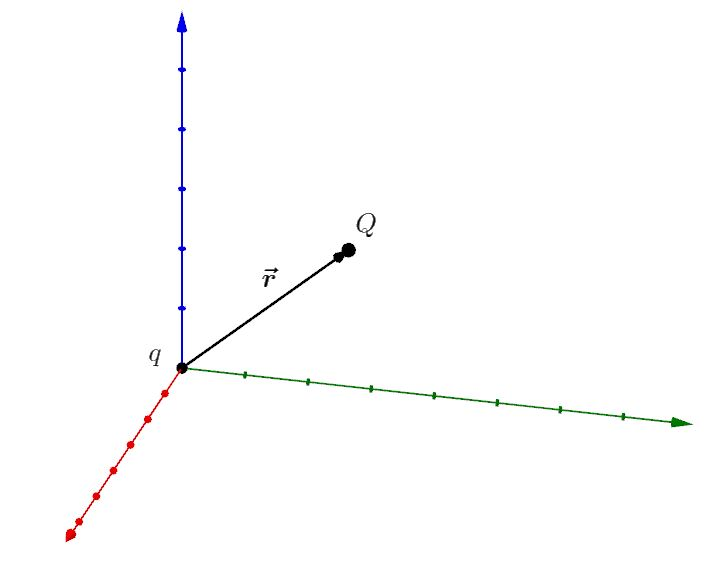
\includegraphics[scale=0.55]{Elektro/emfig/fig1.JPG}
    \caption{Vektoren $\va{r}$ vises her, hvor $\vu{r}$ har samme retning, men bare kortere med en længde på 1.}
    \label{em:fig:fig1}
\end{figure}

Vi har positive og negative ladninger, hvilket vises med et fortegn (eks. $q=+\SI{1}{\coulomb}$ positiv, $q=-\SI{1}{\coulomb}$ negativ, hvor $\SI{}{\coulomb}$ er enheden for ladning: Coloumb). Hvis produktet af ladningerne er positivt ($Qq>0$), så har vi en frastødning. I det tilfælde vil $\va{F}$ pege i samme retning som $\va{r}$. Hvis produktet i stedet er negativt ($Qq<0$), så vil vi have tiltrækning, og $\va{F}$ vil  pege i modsat retning af $\va{r}$.

Dernæst vil vi gerne introducere en vektor, der ligesom $\va{r}$ tegner en vektor fra $q$ til $Q$, men fra et vilkårligt koordinatsystem, altså med origo vilkårligt placeret). Dette kan lyde lidt mystisk, og endda besværligt, men det vil være en stor hjælp i sidste ende. Denne vektor er:
%
\begin{align}
    \va{R}=\va{r}-\va{r}',
\end{align}
%
hvor $\va{r}'$ går fra origo til $q$, $\va{r}$ går fra origo til $Q$. Derved går $\va{R}$ fra $q$ til $Q$. Dette ses også på \cref{em:fig:fig2}.
%
\begin{figure}[]
    \centering
    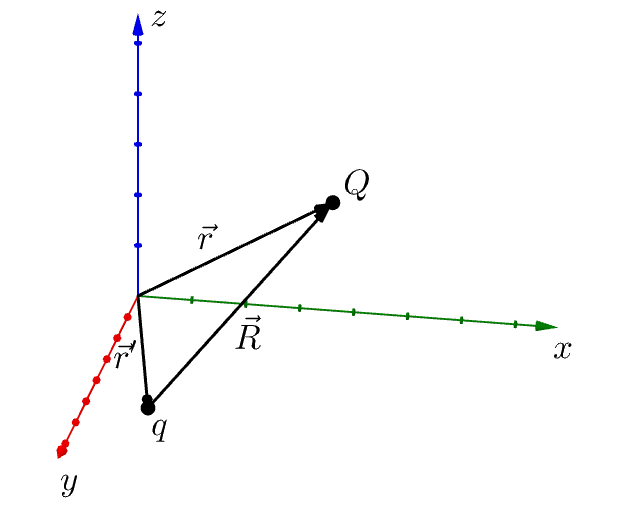
\includegraphics[scale=0.6]{Elektro/emfig/fig2.PNG}
    \caption{Positionsvektorer af $q$ og $Q$ i et vilkårligt koordinatsystem}
    \label{em:fig:fig2}
\end{figure}
%
I et tilfældigt koordinatsystem er Coloumbs lov dermed givet ved
%
\begin{align}
    \va{F}=\frac{1}{4\pi\epsilon_0}\frac{Qq}{R^2}\vu{R} \qquad \text{eller} \qquad \va{F}=\frac{1}{4\pi \epsilon_0}\frac{Qq}{R^3}\va{R},
\end{align}
%
hvor det igen er brugt, at $\va{R}=R\vu{R}$.

Den sidste omskrivning vi vil lave, er, at vi fjerner størrelsen $Q$ fra Coloumbs lov. Grunden til at vi gør dette, er ikke umiddelbart intuitiv, så derefter vil vi se, om ikke vi kan få mening ud af det. Fra dette fås en størrelse, der hedder det \emph{elektriske felt} eller blot $E$-feltet:
%
\begin{align} \label{em:eq:efelt_def} 
    \va{E} = \frac{\va{F}}{Q} = \frac{1}{4\pi \epsilon_0}\frac{q}{R^2}\vu{R}.
\end{align}
%
Alt vektorregning fra \cref{em:fig:fig2} vil bære over, bortset fra at punktladningen $Q$ vil forsvinde fra tegningen. Det vi har nu, er ikke en kraft, og kræver derfor lidt omtanke. Man kan overveje følgende: Hvis vi i et koordinatsystem kun har en ladning $q$, så er der intet, $q$ kan udføre en kraft på. Der altså ingen kræfter tilstede. Jamen, hvad er så tilstede? Det elektriske felt! $E$-feltet er et form for elektrisk landskab, der tegnes for alle positioner i rummet grundet $q$s eksistens. Hvad betyder E-feltet så? Jo, det fortæller dig i hvilken retning, og med hvilken styrke, en testladning $Q$ \emph{ville} skubbes, hvis den placeres det. Hvis du så gerne vil se skubbet, så skal du placere din ladning $Q$ i E-feltet (og anvende $\va{F}=\va{E}Q$).

Man kan så spørge sig selv: hvordan kan det være, at det er smart at introducere dette E-felt, som er en mere abstrakt størrelse? Hvorfor ikke bare arbejde med kræfter? Det elektriske felt giver et mere generelt overblik over den fysiske situationen. Vi behøver ikke overskue de enkelte vekselvirkninger imellem ladninger, men vi betrager i stedet et større billede. Dette er især belejligt, når vi har store, komplekse systemer med mange bestanddele.

\subsection{Ladningstætheder}
Nu har vi introduceret punktladninger og det elektriske felt, som de skaber. Punktladninger er dog blot en approksimation. Det er begrænsende at skulle approksimere alt til et punkt, og vi vil derfor udvikle nogle nye værktøjer, til at kunne beskrive flere virkelige objekter (såsom en ledning, en ladet flade eller en ladet kasse). Vi introducerer nogle nye størrelser:
%
%og fysikere kan godt lide at beskæftige sig med fænonemer som vi kan beskrive ud fra en teori, hvorefter vi rent faktisk kan gå ud i den store hvide verden og \emph{måle}, om vores teori nu passer. Derfor vil vi gerne lige snakke om andre måder, hvorpå man kan have et objekt med en givet ladning.%
%
\begin{itemize}
    \item \emph{Linjeladning, benævnes $\lambda$ og har enheden \si{\coulomb\per\metre}}. Den beskriver 1-dimensional ladning
    \item \emph{overfladesladning, benævnes $\sigma$ og har enhed \si{\coulomb\per\metre\squared}}: Den beskriver 2-dimensional ladning
    \item \emph{Volumeladning, benævnes $\rho$ og har enheden \si{\coulomb\per\metre\cubed}}: Den beskriver 3-dimensional ladning
\end{itemize}
%
Vi har altså 4 forskellige typer ladningstætheder (ladning per volumen eksempelvis), som har 0, 1, 2 eller 3 dimensioner. Teknisk set, er det kun volumeladningen $\rho$, der er realistisk, da vi lever i et tredimensionelt rum, men de andre bruges stadig ofte, hvis man vil opstille en simplere og mere anvendlig model. Til vores brug vil ladningsfordelingerne oftest være \emph{uniforme} (benævnes også konstant), hvilket betyder, at ladningen er fordelt ligeligt over figuren, ligesom glassur på en kage. Hvordan kan vi anskue det E-felt, som hver af disse typer af ladninger udspænder? Til dette kan vi drage inspiration fra punktladninger. Hvis vi havde en samling af punktladninger, og skulle finde ud af hvilket E-felt, de danner sammen, så skal vi lægge hver af deres bidrag til E-feltet sammen:
%
\begin{align} \label{em:eq:e_felt_punktladninger}
    \va{E}=\frac{1}{4\pi\epsilon_0}\sum_{i=1}^{n}\frac{q_i}{R_i^2}\vu{R}.
\end{align}
%
Hvorfor giver det her mening? Lad os lige kigge på to ladninger $q_1$ og $q_2$, hvor de hver skubber til en testladning $q$ med deres respektive kræfter (se \cref{em:fig:fig4}). Den totale kraft, vil dannes som $\va{F}_{total}=\va{F}_1+\va{F}_2$. Det tilsvarende E-felt, som beskriver dette, er dermed
%
\begin{align}
    \va{E} = \frac{\va{F}_{total}}{Q} = \frac{1}{Q} \left( \va{F}_1+\va{F}_2 \right) = \frac{1}{4\pi\epsilon_0} \left( \frac{q_1}{R_1^2}\vu{R}_1+\frac{q_2}{R_2^2}\vu{R}_2 \right),
\end{align}
%
som også er, hvad \cref{em:eq:e_felt_punktladninger} siger. Dette kan også fortolkes lidt, da man kan se det som, at deres elektriske landskaber overlapper med hinanden, og derfor skal de \emph{lægges} sammen.

\begin{figure}[]
    \centering
    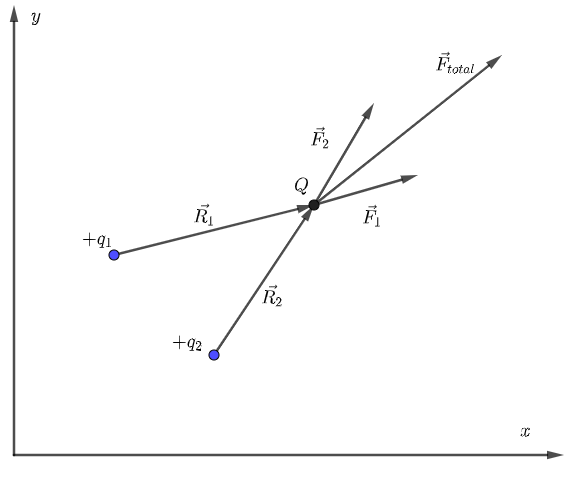
\includegraphics[scale=0.55]{Elektro/emfig/fig4.PNG}
    \caption{Påvirkning af testladningen $Q$ fra to punktladninger $q_1$ og $q_2$.}
    \label{em:fig:fig4}
\end{figure}

Nu til at finde E-feltet af vores nye ladningstætheder. Til dette vil vi igen summere kilderne til det elektriske felt sammen, men hvad er vores kilder? Det er uendelig små versioner af den relevante ladningstæthed. Har vi eksempelvis en linjeladning $\lambda$ med længde $L$, så kan den opdeles i mange små stykker af størrelsen\footnote{Grunden til at vi sætter et $'$ på $\dd{l}$'et, er fordi $'$ bruges til objekter, der henviser til ladningen af systemet, præcis ligesom i \cref{em:fig:fig2} med $\va{r}'$} $\dd{l}'$. Hvert af disse små stykker har en ladning $\lambda\dd{l'}=\dd{q}$. Hvis vi ville have det samlede E-felt, så skal vi summere alle disse små bider, ligesom vi gjorde med punktladninger i \cref{em:eq:e_felt_punktladninger}. I forhold til overfladesladning og volumeladning skal man summere over $\sigma\dd{a'}=\dd{q}$ og $\rho\dd{V'}=\dd{q}$. Men når man summere over infinitesmale størrelser, så bruger man integralregning til at bestemme summen. %Så vi vil skrive summen om til et integrale (men det er bare en sum!).
Helt generelt har vi, at

\begin{align}
    \va{E} &= \frac{1}{4\pi\epsilon}\int\frac{1}{R^2}\vu{R}\dd{q}, \label{em:eq:e_felt_densitet}
    %
    \intertext{hvilket kan skrives om til et af de 3 ladningstætheder.}
    %
    \va{E} &= \frac{1}{4\pi\epsilon}\int\frac{\lambda}{R^2}\vu{R}\dd{l'}, \label{em:eq:e_felt_densitet_1d} \\
    \va{E} &= \frac{1}{4\pi\epsilon}\int\frac{\sigma}{R^2}\vu{R}\dd{a'}, \label{em:eq:e_felt_densitet_2d} \\
    \va{E} &= \frac{1}{4\pi\epsilon}\int\frac{\rho}{R^2}\vu{R}\dd{V'}. \label{em:eq:e_felt_densitet_3d}
\end{align}
%
Det er gået lidt stærkt med gennemgangen af metoden til at opstille E-feltet for de forskellige ladningstætheder. Det er fordi, vi ikke rigtigt kommer til at bruge det (bortset fra en enkelt opgave). Det, der er vigtigt at tage med fra dette afsnit, er, at der er forskellige ladningstætheder, og at man vha. kan integralregning finde det E-felt de udspænder. Men det er ikke fokusset af dette emne, at regne disse integraler.

\subsection{Symmetrier}
% I princippet, så er vi \emph{færdig} med elektrostatik.
Med ladningstæthedsintegralerne ovenover, \cref{em:eq:e_felt_densitet,em:eq:e_felt_densitet_1d,em:eq:e_felt_densitet_2d,em:eq:e_felt_densitet_3d}, kan vi konstruere en hvilket som helst ladningskonfiguration, og finde det E-felt, det udspænder. Så kan vi sætte en ladning ned, hvor vi har lyst, og se, hvordan den påvirkes af E-feltet. Desværre er disse integraler ofte meget indviklet at bestemme. Som fysikere, så leder man tit efter, hvordan man kan gøre noget smartere. Favoritværktøjet til dette er at bruge symmetri. Her snakker vi om symmetri i sin bredeste forstand, der findes flere forskellige slags. Symmetri er når man kan påvirke et system på en eller anden måde, uden at ændre systemet: En cirkel er f.eks. rotationssymmetrisk, fordi den kan roteres den halv omgang, hvorefter den stadig er samme cirkel.
Det egentlige formål med dette emne er altså, at illustrere anvendelse af symmetri, så lad os se noget symmetri.

\subsubsection{Gauss' lov}
Dejlig symmetri falder desværre ikke bare ned fra himlen. Vores system er elektriske felter, der skabes af ladninger: spørgsmålet er så om, vi kan udnytte denne sammenhæng? Det kan man, og til det, vil %jeg anvende en ``matematisk'' måde at måle på et elektrisk felt. Dette kaldes flux. 
vi definere en størrelse kaldet elektrisk flux:
%Lad os prøve at kigge lidt på hvilken størrelse det er. Matematisk er det givet ved:
%
\begin{align}
    \Phi_\textup{E}=\oint \va{E}\cdot \dd{\va{a}}.
    \label{eqm:eq:flux}
\end{align}
%
\Cref{eqm:eq:flux} indeholder et såkaldt ``lukket integral'', der har symbolet $\oint$. Det betyder at man skal integrere over en lukket overflade, eksempelvis overfladen på en kuglen eller en kasse. Hvordan dette gøres gemmes for nu til senere. %Det ser allerede lidt sjovt ud. Så før jeg går ned i dybden med matematikken, så vil jeg prøve at give en intuitive forklaring for flux.
Flux kan tænkes som et mål for, hvor meget det elektriske felt peger ud gennem en overfladen\footnote{I gammel literatur ser man ofte det elektrisk felt omtalt som elektrisk fluxtæthed eller fluxdensitet, da det elektriske felt er for den elektriske fluxm hvad massefylde eller densitet, er for massen af et objekt.}.% Men det lyder allerede underligt. Kan E-feltet nu strømme? Før var E-feltet beskrevet som et elektrisk landskab, men f
Forestil dig følgende: Du ser et landskab (et rigtigt landskab) foran dig. 
% Men hvordan kan det være, at du ser det landskab? Jamen 
Vi ser landskabet ved at lys er rejst fra positioner i rummet til din lokation. %for at fortælle dig om, hvordan landskabet ser ud. 
Holder du nu en plan overflade, eksempelvis en glasplade, op foran dit udsyn, så vil lyset strømme igennem overfladen, og derefter hen til dig. Igennem overfladen må der passere forskellige mængder af fx. rødt, grønt og blåt lys, og de må komme fra forskellige vinkler. Sammen tegner de et landskab for dine øjne, som på den plane overflade tegner et billede af hvordan landskabet ser ud.
% (Ja, dine øjne er en del sejere end en overflade).
Det er det, der er formålet med flux. Vi holder en overflade oppe, og får derved en ide om, hvordan det elektriske landskab (E-feltet) ser ud. Se også \cref{em:fig:landskab}.
% Med det sagt, så er vores opgave rent faktisk nemmere end at finde fluxen af et decideret lys-landskab, da vi kun har én kilde (ladning), der udsender et slags information (E-felt). Dette kunne eks. sammenlignes med, hvis der kun fandtes rødt lys med bølgelængde 652nm og dette udgjorde udelukkende landskabet. Så på samme måde som fotonerne skaber et visuelt landskab, så skaber E-felter et elektrisk landskab. Så måden vi "måler" det elektriske landskab er ud fra det elektriske felt, mens det er fotoner for et almindeligt landskab. Så flux er spændende fordi det kan fortælle os rigtig meget om hvilket slags elektrisk felt vi har med at gøre!

\begin{figure}[]
    \centering
    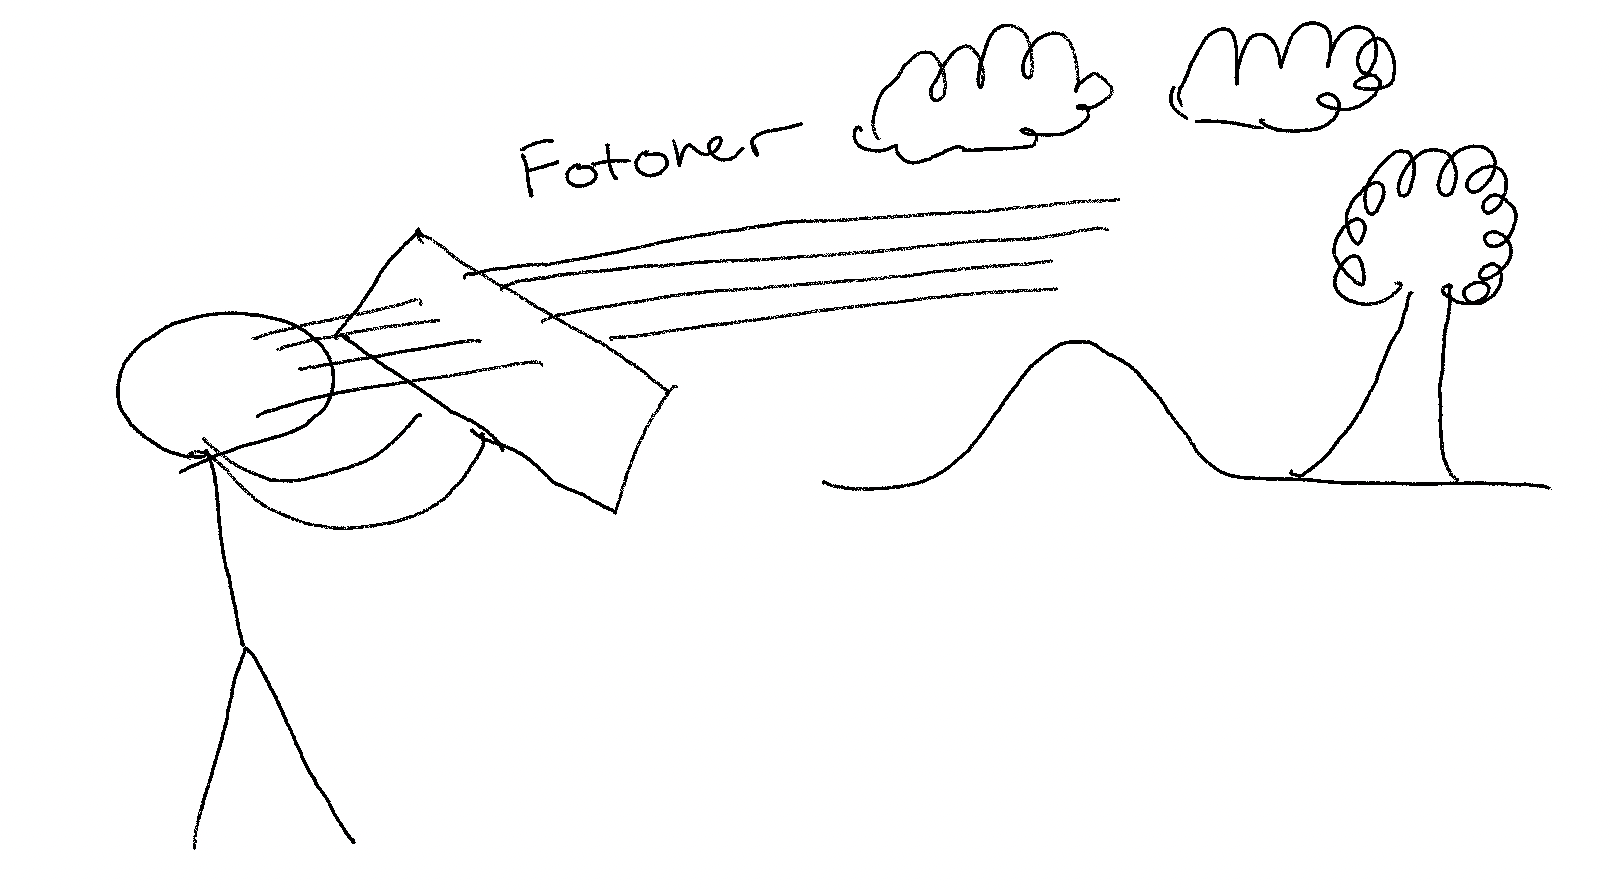
\includegraphics[scale=0.45]{Elektro/emfig/landskab.png}
    \caption{Illustration af hvordan flux kan tænkes. Fluxen igennem glaspladen beskriver hvor meget lys, der passerer igennem pladen, og derved hvor meget lys personen ser.}
    \label{em:fig:landskab}
\end{figure}

Nu er det tid til at forklare matematikken bag ligning (\ref{eqm:eq:flux}). Vi nævnte at det er lukket overfladeintegrale. Det indebærer, at man summerer over en overflade, der er lukket (eksempelvis overfladen af en kasse eller en sfære). Det betyder altså, at vi kan gøre det bedre, end at holde en plan overflade oppe. Vi vil i stedet omringe det elektriske landskab med en lukket overflade, og derved få et godt billede hele vejen rundt.% (lidt ligesom en snekugle omringer eks. et juletræ med en sfære).
Sådan kan vi garantere et fuldendt billede. Dernæst ser vi, at $\va{E}\cdot \dd{\va{a}}$ er et prikprodukt. Den infinitesmale vektor $\dd{\va{a}}$ skal forstås som en vinkelret vektor på den infinitsmale overflade $\dd{a}$, og kan generelt omskrives til
%
\begin{align}
    \dd{\va{a}}=\dd{a}\vu{n}.
\end{align}
%
Her $\vu{n}$ er en enhedsvektor, som er vinkelret på overfladen $\dd{a}$. Se \cref{em:fig:davektor} for en illustration af dette.
%
\begin{figure}
    \centering
    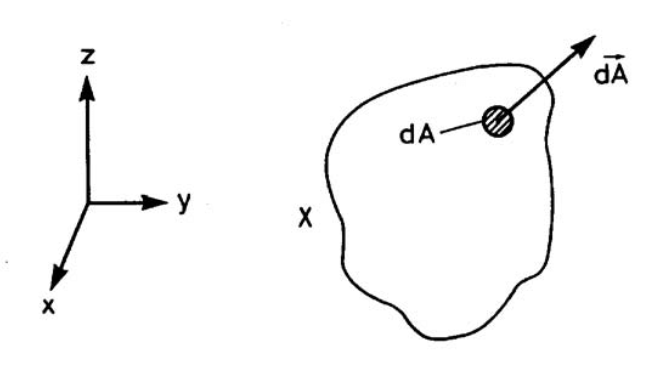
\includegraphics[scale=0.5]{Elektro/emfig/fig5.PNG}
    \caption{$\dd{a}$ er et infinitsmalt areal, hvor $\dd{\va{a}}$ er en infinitsmal vektor vinkelret på arealet $\dd{a}$. Kilde: \cite{DefinitionAreaVector}.}
    \label{em:fig:davektor}
\end{figure}
%
Dette prikprodukt er vores måde at tage højde for hvilken retning E-feltet peger igennem overfladen. Det er vigtigt at kende denne retning, for at få det rigtige billede.

Lad os prøve at se på et simpelt eksempel, for at få en fornemmelse af alt dette. E-feltet antages at være konstant og på formen $\va{E} = E_0\vu{x}$, hvor $E_0$ er en konstant. Vi vil nu finde fluxen. Nu er det vores opgave at konstruere en lukket overflade, og derved ``måle'' fluxen gennem denne. Det simpleste, vi kan vælge, er overfladen af en kasse. Den har seks overflader, og vi kan derfor dele integralet op i 6 integraler -- en for hver overfalde på kassen -- ved at bruge sumreglen for integralregning fra \cref{mat:sec:intergral}:

\begin{figure}[]
    \centering
    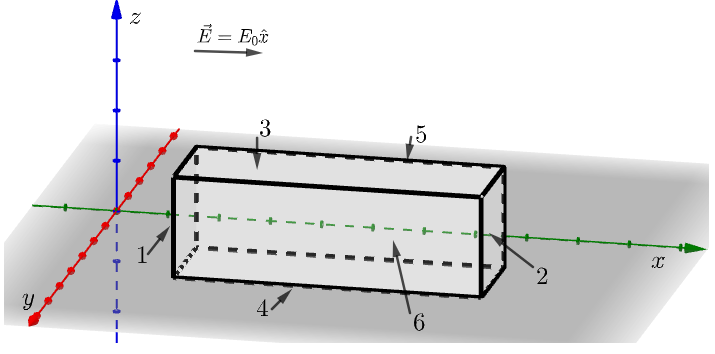
\includegraphics[scale=0.75]{Elektro/emfig/fig3.PNG}
    \caption{En lukket overflade i form af en kasse til at måle fluxen af et konstant E-felt.}
    \label{em:fig:em:fig:overfladeintegral_kasse}
\end{figure}

\begin{align} \label{em:eq:overfladeintegral_kasse}
    \oint \va{E}\cdot \dd{\va{a}}=\int_1 \va{E}\cdot \dd{\va{a}}+\int_2 \va{E}\cdot \dd{\va{a}}+\int_3 \va{E}\cdot \dd{\va{a}}+\int_4 \va{E}\cdot \dd{\va{a}}+\int_5 \va{E}\cdot \dd{\va{a}}+\int_6 \va{E}\cdot \dd{\va{a}}.
\end{align}
%
I \cref{em:eq:overfladeintegral_kasse} henviser tallene på integralerne til overfladerne af samme nummer i \cref{em:fig:em:fig:overfladeintegral_kasse}, der illustrerer situationen. Fire af disse overflader er beskrevet af en vektor, $\dd{\va{a}}$, der peger i $y$- eller $z$-retningen. Disse er vinkelrette med E-feltet, som peger i $x$-retningen. Vi husker fra \cref{mat:sec:intergral} at prikproduktet for to vinkelrette vektorer er nul. Det betyder, at overfladerne 3 til 6 alle bliver integralet af nul, der i sig selv er nul. Med formelsprog er dette for overflade 3
%
\begin{align}
    \int_3 \va{E}\cdot \dd{\va{a}} = \int 0 \dd{a} = 0,
\end{align}
%
hvilket betyder at
%
\begin{align}
    \oint \va{E}\cdot \dd{\va{a}}=\int_1 \va{E}\cdot \dd{\va{a}}+\int_2 \va{E}\cdot \dd{\va{a}}.
\end{align}
%
Nu kan vi indsætte $\dd{\va{a}}=\pm\dd{a}\vu{x}$ for henholdsvis overflade 1 og 2, samt at $\va{E}=E_0\vu{x}$:
%
\begin{align}
    \oint \va{E}\cdot \dd{\va{a}}=\int_1 E_0\vu{x}\cdot(-\dd{a}\vu{x}) +\int_2 E_0\vu{x}\cdot \dd{a}\vu{x}=\int_2 E_0\dd{a}-\int_1 E_0\dd{a}.
\end{align}
%
Da $E_0$ er konstant, så kan den sættes udenfor integralerne, og så har vi tilbage at
%
\begin{align}
    \oint \va{E}\cdot \dd{\va{a}}=E_0\int_2\dd{a}-E_0\int_1\dd{a}.
\end{align}
%
Her kommer så punktet, hvor vi ikke behøver at beregne integralet. I \cref{mat:subsec:int} så vi, at integralet svarer til at lægge en masse små elementer sammen. Integralet $\int_1\dd{a}$ er derfor resultatet af at lægge arealet af en masse små dele af overflade 1 sammen, hvilket er arealet af hele overflade 1. Kalder vi det areal A, og bemærker at overflade 2 også have samme areal, så får vi resultatet:
%
\begin{align}
    \oint \va{E}\cdot \dd{\va{a}}=E_0A-E_0A=0.
\end{align}
%
Hvad betyder det så at fluxen her er nul? % Men hvad med E-feltet? Jo, det der er sket her er, der er strømmet 
Svaret er, at der er ligeså meget af E-felt, der peger ind i kassen igennem overflade 1, som peger ud af kassen ved overflade 2. Fluxen fortæller os derfor, at hele den del af det elektriske felt, der kommer ind i kassen, også går ud af kassen et andet sted. Der er med andre ord ikke fanget noget inde i kassen.
% Er det pga. vores dårlige valg af overflade? Nej ikke helt. Vores problem er nærmere, at inde i vores overflade er der ingen kilder til E-feltet, så E-felter er bare suset forbi. Der er ingen afløb som E-feltet bliver suet ned i, eller E-felter som pludseligt opstår. Men E-feltet må komme fra et eller andet sted? Ja det er sandt, og jeg har snydt lidt her for forståelsens skyld. Man kan tænke på det som, at jeg har begrænset, hvor vi kan sætte vores overflade. Og i dette rum er $\va{E}=E_0\vu{k}$.

For at se på et eksempel, hvor fluxen ikke er nul, vil vi nu finde fluxen fra en punktladning i origo. Her er E-feltet
%
\begin{align}
    \va{E} = \frac{1}{4\pi\epsilon_0}\frac{q}{r^2}\vu{r}=|E|\vu{r},
\end{align}
%
hvor
%
\begin{align}
    |E| = \frac{1}{4\pi\epsilon_0}\frac{q}{r^2}.
\end{align}
%
En praktisk overflade at vælge i dette tilfælde, er en sfære med centrum i origo med radius $R_0$ (se \cref{em:fig:fig6}). Da vil $\dd{\va{a}}$ altid være parallelt med E-feltet, fordi det elektriske felt peger væk fra origo, mens $\dd{\va{a}}$ er vinkelret på overfladen af sfæren, hvilket er retningen væk fra centrum. Skrives arealelementvektoren som $\dd{\va{a}}=\dd{a}\vu{r}$ kan fluxen beregnes som
%
\begin{figure}
    \centering
    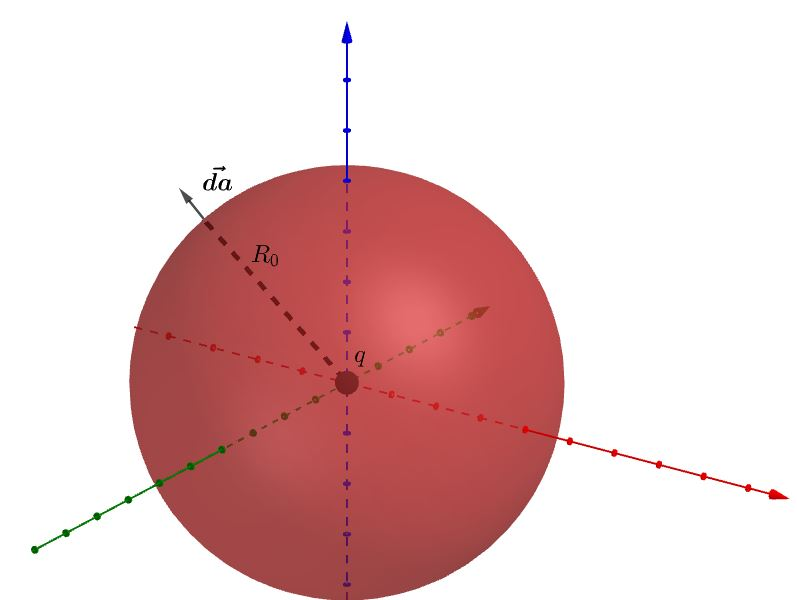
\includegraphics[scale=0.5]{Elektro/emfig/fig6.JPG}
    \caption{Flux af en punktladning igennem en sfære med radius $R_0$.}
    \label{em:fig:fig6}
\end{figure}
%
\begin{align}
    \oint\va{E}\cdot\dd{\va{a}} = \oint |E|(\vu{r}\cdot\vu{r})\dd{a} = \oint |E|\dd{a},
\end{align}
%
da $\vu{r}\cdot\vu{r} = 1$. Men vi kan se, at $|E|$ kun afhænger af afstanden $r$ fra centrum, hvorfor $|E|$ er den samme i 
%. Og hvis vi summerer over en sfære overflade med radius $R_0$, så vil $|E|=\frac{1}{4\pi\epsilon_0}\frac{q}{R_0^2}$ i 
alle punkter på sfærens overfladen. $|E|$ er derfor em konstant i integralet, som kan sættes udenfor integralet:
%
\begin{align}
    \oint\va{E}\cdot\dd{\va{a}}=|E|\oint\dd{a}.
\end{align}
%
Da $\oint\dd{a} = A$ er overfladearealet af sfæren, hvilket er
%
\begin{align}
    A = 4\pi R_0^2,
\end{align}
%
bliver fluxen
%
\begin{align}
    \Phi_\textup{E} = \oint\va{E}\cdot\dd{\va{a}} = \frac{1}{4\pi\epsilon_0}\frac{q}{R_0^2}4\pi R_0^2=\frac{q}{\epsilon_0}.
\end{align}
%
Nu er vi kommet frem til det spændende resultat: fluxen er lig med punktladningen $q$ divideret med en konstant $\epsilon_0$. Hvad er det helt præcist, vi har gjort for at komme frem til det? Vi har placeret en ladning $q$ i origo, bestemt fluxen gennem en lukket overflade, der indkapsler ladningen $q$, og fundet ud af, at fluxen afhænger direkte af $q$. I det første tilfælde med kassen uden ladning, var fluxen 0. Fluxen fortæller os derfor hvor meget ladning, der er inde i en lukket overflade! Vi kunne have ligeledes sat to punktladninger $q$ inde i vores sfære, og vi ville være kommet frem til at fluxen så er
%
\begin{align}
    \Phi_\textup{E} = \oint\va{E}\cdot\dd{\vu{a}} = 2q/\epsilon_0.
\end{align}
%
Det vi er kommet frem til gælder generelt og hedder Gauss' lov:
%
\begin{align} \label{em:eq:gauss}
    \oint \va{E}\cdot \dd{\va{a}}=\frac{Q_\textup{inde}}{\epsilon_0}.
\end{align}
%
Hvor $Q_\textup{inde}$ er den indsluttede ladning. Jo mere ladning vi samler inde i vores lukket overflade, desto mere flux. Derudover kaldes disse lukkede overflader for \emph{Gaussoverflader}, og vi vil bruge det udtryk fremover. Gauss' lov er en relation, som vi faktisk kan udnytte, til at bestemme E-feltet, hvis vi har noget symmetri, at støtte os til. Dette er nok nemmest at vise med nogle eksempler, så det vil vi gøre med det samme.

\begin{figure}[]
    \centering
    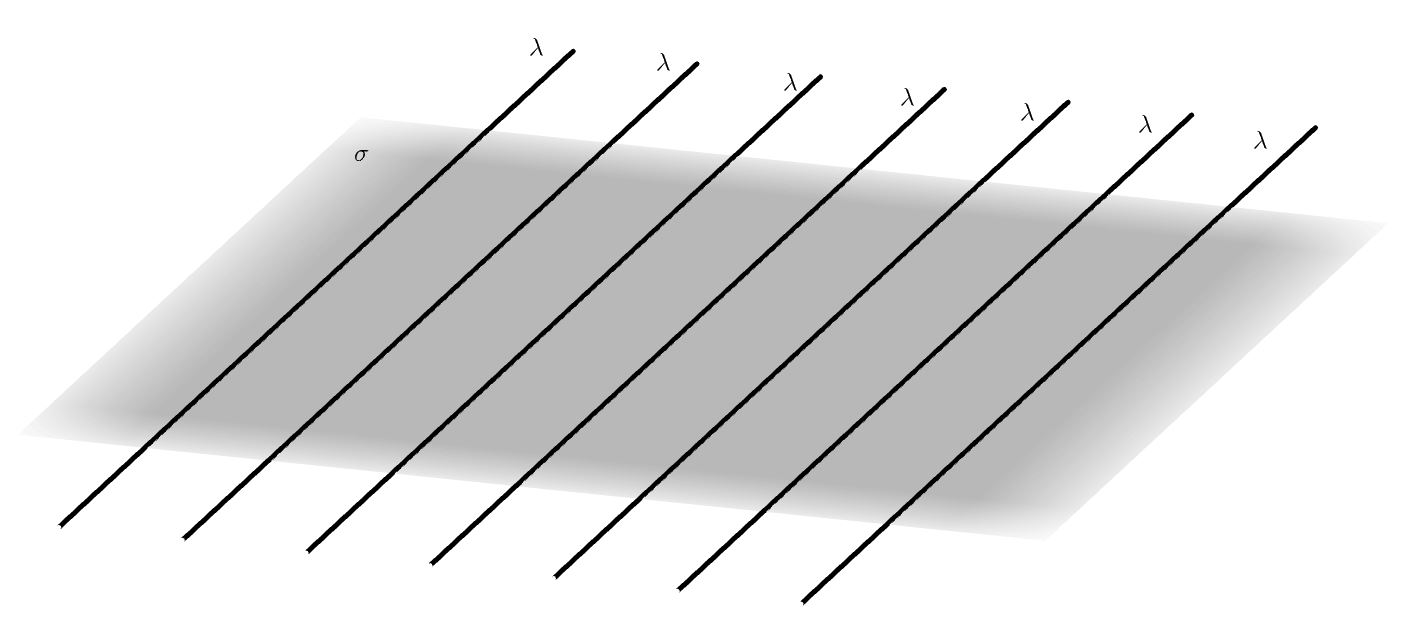
\includegraphics[scale=0.4]{Elektro/emfig/sym12.JPG}
    \caption{På figuren er der mellemrum mellem linjerne, men det er bare så kan man se linjerne. Det er meningen, at linjerne skal ligge helt oppe ad hinanden og konstruere pladen.}
    \label{em:fig:ladet_plan}
\end{figure}
%
\subsubsection{Plansymmetrisk E-felt}
Det første eksempel, vi vil kigge på, er en uendelig lang og bred plade med konstant overfladeladningstæthed $\sigma$. Vi kan bruge symmetri til at bestemme retningen på E-feltet. %Men allerede dette er lidt uoverskueligt, så endnu simplere er at splitte 
Hertil hjælper det at dele pladen op i mange uendelige lange linjer med linjeladningstætheden $\lambda$, som ligger helt op ad hinanden. De vil tilsammen udgøre pladen, hvilket er illustreret i \cref{em:fig:ladet_plan}.
%
% Okay, en uendelig lang ladet linje, er stadig lidt svært at anskue. Helt basalt skal vi nok starte med at kigge på en endelig linje med konstant linjeladning $\lambda$. Men for at betragte symmetrien bag dette, så er det konceptuelt nemmere at anse 
For at forstå den uendeligt lange linje, er det en god idé at starte med punktladninger jævnt fordelt på en linje. Lad os betrage 3 sådanne ladninger, hvilket er illustreret i \cref{em:fig:sym1/2}.
%
Placeres en testladning $q$ midt over linjeladningen, så vil vi se en simpel påvirkning. Ud fra symmetrien kan vi sige, at $\va{F}_1$ og $\va{F}_3$'s vandrette komposanter gå ud med hinanden, mens $\va{F}_2$ ikke har en vandret komposant. Resultatet bliver, at $q$ bare skubbes direkte lodret op, se \cref{em:fig:sym1/2}.
%
\begin{figure}[]
    \begin{minipage}{0.5\textwidth}
        \center{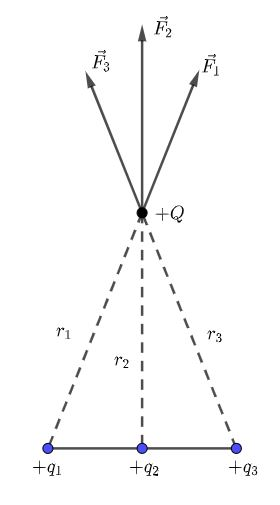
\includegraphics[scale=0.5]{Elektro/emfig/sym1.JPG}}
    \end{minipage}\hfill
    \begin{minipage}{0.5\textwidth}
        \center{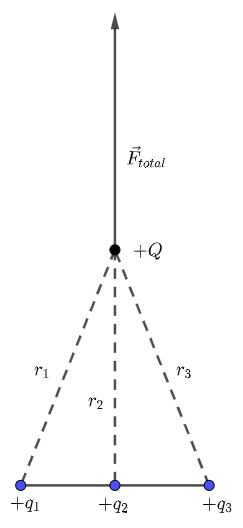
\includegraphics[scale=0.5]{Elektro/emfig/sym2.JPG}}
    \end{minipage}\hfill
    \caption{De 3 ladninger sidder fast på en linje. De vandrette komposanter af den totale kraft går parvist ud med hinanden, så den totale kraft peger vinkelret væk fra linjen.}
    \label{em:fig:sym1/2}
\end{figure}
%
Hvis vi forlænger linjeladningen, og samtidig beholder $Q$s position, så har vi stadig, at den totale kraft påvirkning er lodret (\cref{em:fig:sym3}). Det er fordi symmetrien er bevaret.
%
\begin{figure}[]
    \centering
    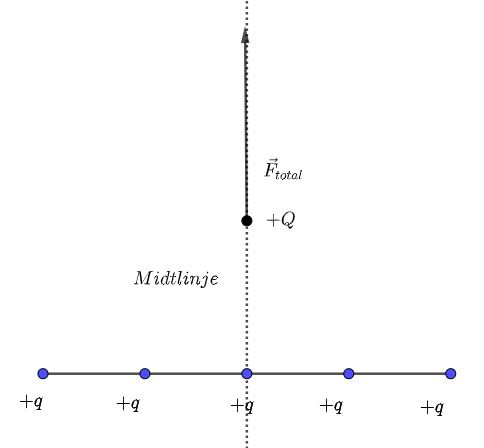
\includegraphics[scale=0.65]{Elektro/emfig/sym3.JPG}
    \caption{Tilføjes flere ladninger til \cref{em:fig:sym3}, således at symmetrien er bevaret, vil det stadig være sandt, at den totale kraftpeger vinkelret væk fra linjen.}
    \label{em:fig:sym3}
\end{figure}

Nu vil vi prøve at lege med symmetrien. Rykkes $q$ en smule til højre. Så har vi ikke længere, at den totale kraftpåvirkning er lodret (se \cref{em:fig:sym4}).
%
\begin{figure}[]
    \centering
    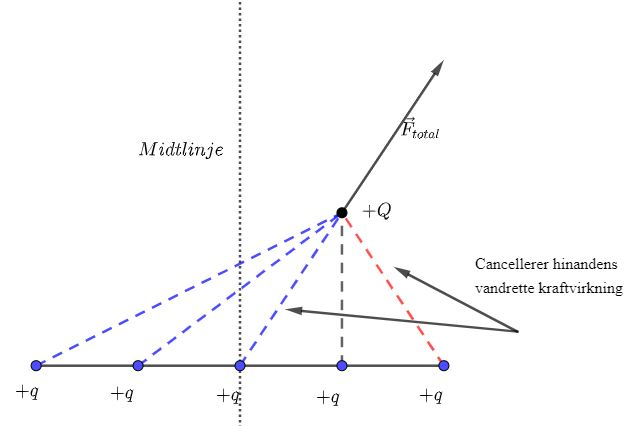
\includegraphics[scale=0.7]{Elektro/emfig/sym4.JPG}
    \caption{Brydes symmetrien fra \cref{em:fig:sym1/2,em:fig:sym3} ophører kraften med at pege vinkelret væk fra linjen. Overskudet af ladninger til venstrå for $Q$, får den totale kraft til at blive afbøjet mod højre.}
    \label{em:fig:sym4}
\end{figure}
%
I stedet vil den pege skråt op til højre. Det er fordi de to ladninger til højre og venstre for $q$ vil udligne hinandens vandrette komposanter, og tilsammen vil de bidrage til at skubbe testladningen lodret op. Det samme gør ladningen lige over for $Q$. Tilbage er der de to ladninger ude til venstre, og de vil skubbe $Q$ skråt op til højre.
% Okay, lad os forlænge linjeladningen igen.
Tricket, der gør det muligt at håndtere den uendelige linje, er nu at indse, at alle punkter på linjen kan kaldes midtpunktet. Da linjen er uendelig, kan vi vælge et hvilket som helst punkt på linjen, og uanset hvilket punkt vi vælger, da vil vi have en uendelig lang linje på hver side af os. Vi har lige fundet frem til, at hvis $Q$ placeres midt på en linje med jævnt fordelt ladning, så peger den totale kraft vinkelret væk fra linjen. Når alle punkter på den uendelig linje kan kaldes midtpunktet, så må kraften pege vinkelret væk fra linjen alle steder i rummet. At dette er sandt er netop en konsekvens af at linjen er uendelig lang, og det er en tankegang, der godt kan tage lidt tid at vænne sig til.

% \begin{figure}[]
%     \centering
%     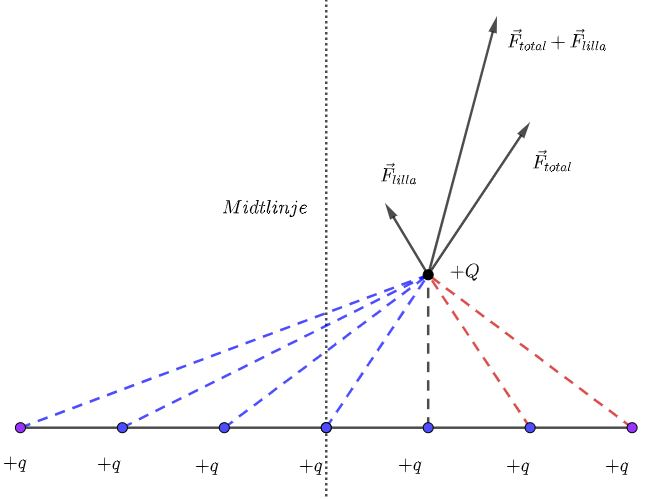
\includegraphics[scale=0.5]{Elektro/emfig/sym5.JPG}
%     \caption{}
%     \label{em:fig:sym5}
% \end{figure}

% De tidligere blå-farvede ladninger vil give den samme kraft $\va{F}_{total}$ mens de to nye lilla ladninger bidrager med $\va{F}_{lilla}$\footnote{Det kan godt være lidt svært at se hvorfor, $\va{F}_{lilla}$ peger skråt op til venstre. Men på vores figur, kan vi se, at den lilla ladning til højre er tættere på $q$ end den til venstre, så den må give en stærkere kraft og være mest dominerende. Vi kan dermed retfærdigøre, at hvis det hovedsageligt er dens påvirkning der gælder, så vil $\va{F}_{lilla}$ nok pege skråt op til venstre}. Vi kan se på \cref{em:fig:sym5}, at kraften fra de yderlige lilla ladninger, retter den nye totale kraft op og gør den mere lodret.
% Og det jo et spændende resultat! Jeg vil nu hypotesere, at hvis vi så forlænger linjeladningen uendelige mange gange, så vil den nye totale kraft være fuldkommen lodret - ligegyldigt hvor vi placerer ladningen $Q$! Jamen, lad os vise det.

% Vi vil nu forlænge linjen uendeligt i begge side, og samtidigt beholder vi $Q$s position. Nu er vi begyndt at have rigtige mange ladninger på linjen, så vi kan ikke længere tegne $+q$ punktladningerne ind på linjen.

% \begin{figure}[]
%     \centering
%     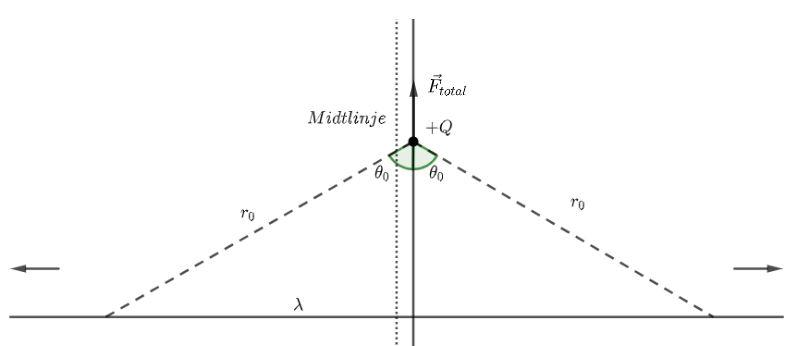
\includegraphics[scale=0.5]{Elektro/emfig/sym6.JPG}
%     \caption{Vi kan blot betragte ladningerne som $r_0$ afgrænser, da de yderligere ladninger vil have en ubetydelig virkning}
%     \label{em:fig:my_label}
% \end{figure}
% For at overskue hvad der nu sker med testladningen $Q$, fokuserer vi kun på de tætteste ladninger på $Q$. Dette kan vi sagtens gøre, fordi de ladninger der ligger for langt væk alligevel bare bidrager med en kraft nær nul (Husk på, at Coloumbs lov aftager med $\frac{1}{r^2}$). Og for at gøre alting nemmere vil vi kigge på de ladninger, der ligger symmetrisk omkring $Q$. Her afgrænser $r_0$ det interval, vi er interesseret i. Distancen $r_0$ bidrager også selv med en kraft nær nul, så det retfærdigører at længere distancer kan ignoreres. Vi kan dermed se, at alle de relevante ladninger ligger symmetrisk om $Q$, så $q$ må nødvendigvis skubbes lodret op. Faktisk kan vi placere $q$ hvor som helst og gøre samme trick - da linjeladningen er uendelig lang! Så vi kan konkludere, at fra en uendelig lang linjeladning, så må E-feltet pege op i alle positioner.

\begin{figure}[]
    % \begin{minipage}{0.5\textwidth}
    %     \center{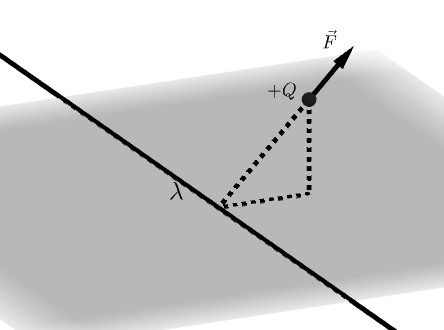
\includegraphics[scale=0.6]{Elektro/emfig/sym7.PNG}}
    % \end{minipage}\hfill
    % \begin{minipage}{0.5\textwidth}
    \centering
    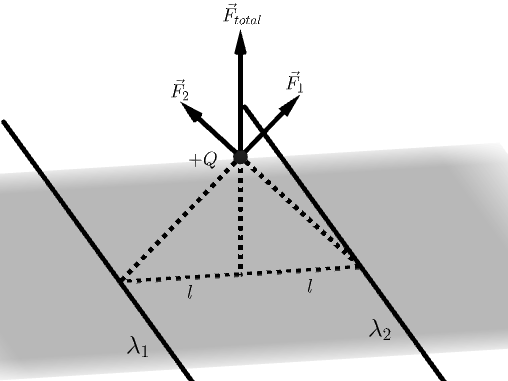
\includegraphics[scale=0.65]{Elektro/emfig/sym8.PNG}
    % \end{minipage}\hfill
    \caption{Den uendelige plan illustreret som grå overflade med den konstante overfladesladningenstætheden $\sigma$. Ligegyldigt hvor testladningen $Q$ placeres, kan vi opdele pladen i par af uendelige linjer, hvis vandrette bidrag til den totale kraft går ud med hinanden.}
    \label{em:fig:sym7/8}
\end{figure}
%
Vi vender nu tilbage til den pladen med den konstante overfladeladningstæthed $\sigma$. Tænker vi på pladen som bestående af uendeligt mange, uendelige lange linjer, så kan vi bruge resultatet fra før: den totale kraft skal pege vinkelret væk fra planen. Vi kan også vise dette argument med en tegning, se \cref{em:fig:sym7/8}. Ligegyldigt hvor testladningen $Q$ placeres over planen, kan vi opdele pladen i par af uendelige linjer, hvis vandrette bidrag til den totale kraft går ud med hinanden. Hvis de vandrette komposanter altid går ud med hinanden parvist, så er der kun én mulig retning tilbage, nemlig vinkelret på planen, hvorfor det må være retningen på den totale kraft. Da den totale kraft og det elektriske felt er parallelle, \cref{em:eq:efelt_def}, vil det elektriske felt også være vinkelret på den uendelige plan.
%Hvis vi placerer $q$ et vilkårligt sted på pladen, så er vi først og fremmest interesseret i hvordan en enkelt vilkårlig linjeladning påvirker den. Vi observerer, at $q$ og linjeladningen $\lambda$ danner et skråplan (\cref{em:fig:sym7/8}).
% Bruger vi vores erfaring fra ovenover, så vil $q$ skubbes langs skråplanen, som det også ses på figuren \ref{em:fig:sym7/8} (venstre side). Nu kan vi finde en anden linjeladning, som har samme vandrette distance $l$ til $q$ på den anden side af $Q$. Summerer vi disse to linjeladningers påvirkninger, da vil de vandrette komponenter gå ud med hinanden, og $q$ vil bare skubbes direkte op (højre side af \cref{em:fig:sym7/8}). Jamen, dette argument kan vi gentage for alle linjeladninger, der udgør pladen. Parvis bliver vi ved med at betragte to linjeladninger, og får altid at deres fælles bidrag vil skubbe $q$ direkte op. Der er lige et særtilfælde, og det er linjeladningen lige under $Q$, men den vil også bare skubbe $q$ direkte op. Altså med andre ord vil E-feltet altid pege lodret op. Samtidigt, hvis vi placerer en ladning $q$ under pladen, så vil situationen bare spejles og E-feltet vil pege lodret ned. Hvad har vi lige gennemskuet igennem symmetri? Jo, at 
E-feltet må derfor kunne skrives som
%
\begin{align} \label{em:eq:efelt_plan_retning}
    \va{E}=|E|\hat{n},
\end{align}
%
hvor $\hat{n}$ er en lidt speciel enhedsvektor, der peger op over pladen, og ned under pladen. $\hat{n}$ kaldes planens normalvektor (normal betyder her ``vinkelret på'').

\begin{figure}[]
    \centering
    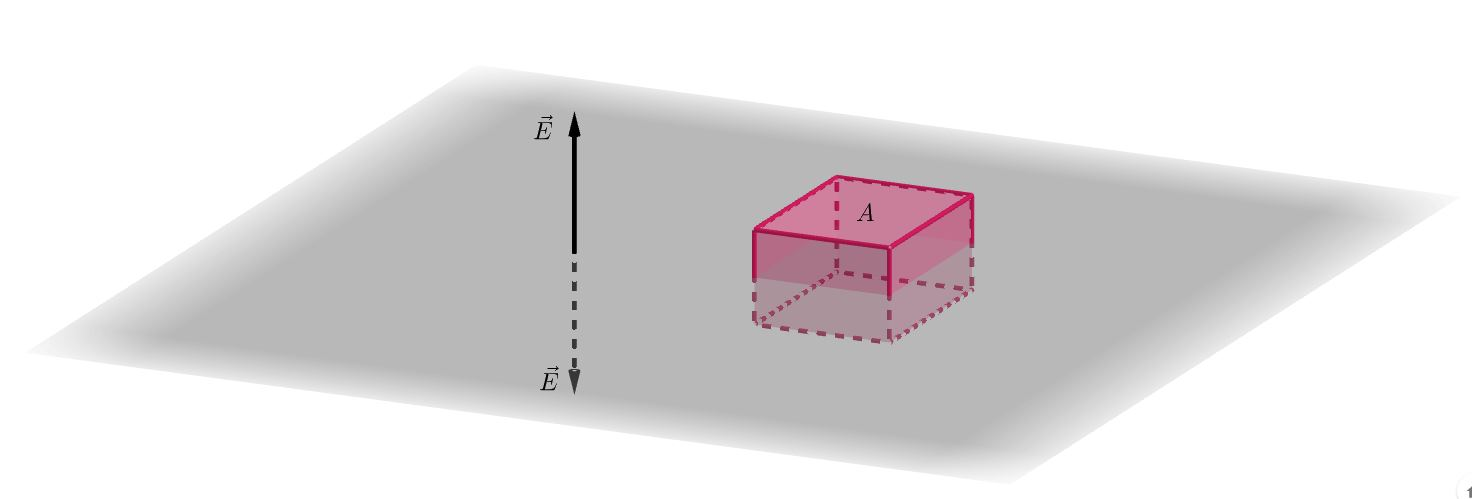
\includegraphics[width=\textwidth]{Elektro/emfig/gaussplan.JPG}
    \caption{Valg af Gaussoverflade for en uendelig stor ladet plade med konstant overfladesladningstæthed $\sigma$. Læg mærke til, at overfladen er ligeså meget over pladen, som den er under.}
    \label{em:fig:plan_gaussoverflade}
\end{figure}

Nu vil vi se, om vi kan udnytte Gauss' lov med disse symmetribetragtninger til at bestemme det elektriske felt fra planen.
%
Gauss' lov, \cref{em:eq:gauss}, siger at
%
\begin{align} \label{em:eq:gauss2}
    \oint \va{E}\cdot \dd{\va{a}} = \frac{Q_\textup{inde}}{\epsilon_0}.
\end{align}
%
Vi vælger nu en kasseformet Gaussoverflade, der rækker ligeså meget over pladen som under pladen, se \cref{em:fig:plan_gaussoverflade}.
%
$\va{E}$ er vinkelret på arealvektoren fra fire af siderne, dem som skærer planen, så deres bidrag til venstresiden af \cref{em:eq:gauss2} vil være 0. Tilbage er der
%
\begin{align}
    \oint \va{E}\cdot \dd{\va{a}} &= \int_\textup{over} \va{E}\cdot\dd{\va{a}} + \int_\textup{under} \va{E}\cdot\dd{\va{a}}.
    %
    \intertext{Vi indsætter nu $\va{E}=|E|\vu{n}$ og får}
    %
    \oint \va{E}\cdot \dd{\va{a}} &= \int_\textup{over}|E|\dd{a}+\int_\textup{under}|E|\dd{a}. \label{em:eq:plan_gauss}
\end{align}
%
På samme måde som alle punkter på en uendelig lang linje er linjens midtpunkt, så er alle punkter i en uendelig plan også planens centrum. Hvis alle punkter er centrum, må vi ikke på nogen måde kunne kende forskel på dem. Det ville vi kunne, hvis det elektriske felt i et punkt afhænger af andet end punktets afstand fra planen. Da de tilbageværende Gaussoverflader er parallelle med planen er $|E|$ derfor en konstant, hvorfor den kan tages udenfor integralet i \cref{em:eq:plan_gauss}.
% Den sidste overvejelse vi vil lave, er, at hvis vi flytter en testladning $q$ i et plan parallelt med pladen (Altså, vi ændrer ikke højden over pladen). Så er $q$ stadig i den samme situation - den befinder sig i samme højde over en uendelig stor ladet plade. Dette kaldes en translationel symmetri (ligesom vi havde roationsymmetri med en cirkel). Ud fra dette må vi kunne sige, at E-feltet må være uændret, da vi ikke har "ændret" på situationen.
% Men intergralerne summere over den øvre og nedre overflade, hvilket er ved en uændret højde. Derfor er |E| \emph{konstant} i integralet. Dette betyder, vi kan hive |E| ud af integralet. 
Tilbage i integralerne er $\int\dd{a}$, hvilket giver arealet $A$. \Cref{em:eq:plan_gauss} bliver således til
%
\begin{align}
    \oint \va{E}\cdot \dd{\va{a}} &= 2|E|A =\frac{Q_\textup{inde}}{\epsilon_0}.
    %
    \intertext{Vi har også, at $Q_\textup{inde}=\sigma A$, da $\sigma$ er overfladeladningstætheden. Dette svarer til at bestemme massen af et objekt ved at gange dets volumen med dets massefylde/densitet. Indsætter vi dette og isolerer $|E|$ fås}
    %
    |E| &= \frac{\sigma}{2\epsilon_0}.
    %
    \intertext{Indsætter dette i \cref{em:eq:efelt_plan_retning}, så har vi at E-feltet er}
    %
    \va{E} &= \frac{\sigma}{2\epsilon_0}\vu{n}.
\end{align}
%
Vi har hermed formået, at udregne E-feltet, udelukkende ved at betragte fluxen gennem en overflade i vores E-felt! Selve resultatet er måske ikke særlig intuitivt: E-feltet er også konstant i alle højder over pladen. Det ville havde været svært at gennemskue, men den er altså god nok\footnote{Det er så svært at finde en real uendelig lang plade at teste det med et eksperiment, men hvis du har en stor nok plade, så kan man sagtens spotte tendensen}. Dette skyldes at ting opfører sig anderledes, når man har med uendeligheder at gøre. Resultatet skyldes derfor antagelsen om at planen er uendelig stor og ikke bare meget stor. Havde man regnet på en meget stor, men endelig plan, så ville feltstyrken rigtignok aftage med afstanden. Det er dog en markant sværere udregning, da man ikke har ligeså meget symmetri at gøre brug af.

\begin{figure}[]
    \centering
    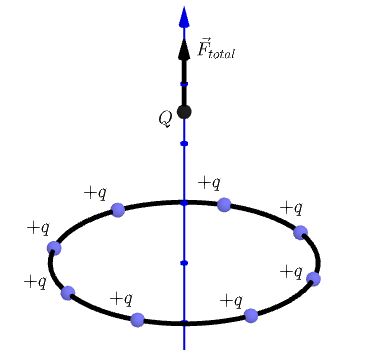
\includegraphics[scale=0.5]{Elektro/emfig/sym10.PNG}
    \caption{Jævnt fordelte ladninger i en cirkel, vil af samme argumenter som for \cref{em:fig:sym1/2,em:fig:sym3}, give, at den totale kraft på en testladning, placeret på aksen gennem cirklens centrum, peger langs aksen.}
    \label{em:fig:cirkelladning}
\end{figure}
%
\subsubsection{Sfærisk symmetrisk E-felt}

Det næste eksempel, vi vil kigge på, er en sfærisk overflade, med centrum i origo, og med radius $R'$, der bærer den konstante overfladesladningstæthed $\sigma$.
%
Det første spørgsmål er så: i hvilken retningen peger E-feltet? Til at overskue dette, så overvejer vi først nogle ligeligt fordelt ladninger placeret på en cirkel. Dette er illustreret i \cref{em:fig:cirkelladning}.
%
Hvis vi så placerer en testladning $q$ over centrum af cirklen, så vil $Q$ skubbes lodret op. Dette skyldes, at for hvert $q$, vil der være et andet $q$ tværs over, der leverer den samme, men modsatrettede, vandrette komposant. Disse vil så gå ud med hinanden, og der vil kun være lodrette komposanter tilbage.
Hvordan bruger vi denne viden til at belyse sfæren? En sfære kan ses som bestående af mange cirkler, men vi bestemmer selv, hvordan vi vil konstruerer sfæren af cirkler. Den mest praktiske måde at konstruere en sfære er symmetrisk omkring en testladning $Q$ (se \cref{em:fig:sym11}).
%
\begin{figure}[]
    \centering
    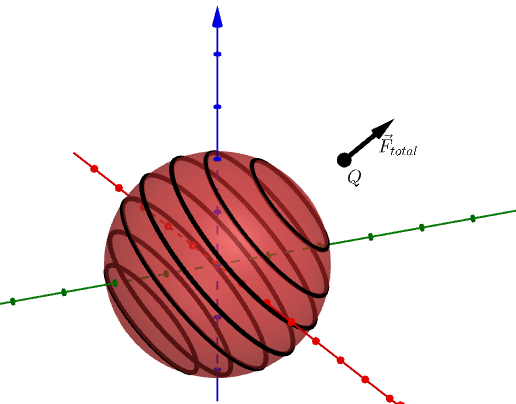
\includegraphics[scale=0.5]{Elektro/emfig/sym11.PNG}
    \caption{Der er mellemrum mellem cirkellinjerne, men det er igen bare for illustrations skyld. Meningen er, at cirkelinjerne skal lægge helt tæt på hinanden og danner en kontinuert sfære.}
    \label{em:fig:sym11}
\end{figure}
%
Hver cirkel (med forskellige størrelser) vil skubbe $q$ den samme vej. Vi kan se, at hver af disse kraftpåvirkninger må pege i samme retning, som en vektor, der går fra centrum til $Q$. Og da $Q$s position er tilfældig (udenfor sfæren), så må det betyde, at E-feltet peger radielt ud fra centrum (ligesom en punktladning!). Vi har altså gennemskuet, at
%
\begin{align} \label{em:eq:efeltstyrke_kugle}
    \va{E}=|E|\vu{r}.
\end{align}

\begin{figure}[]
    \centering
    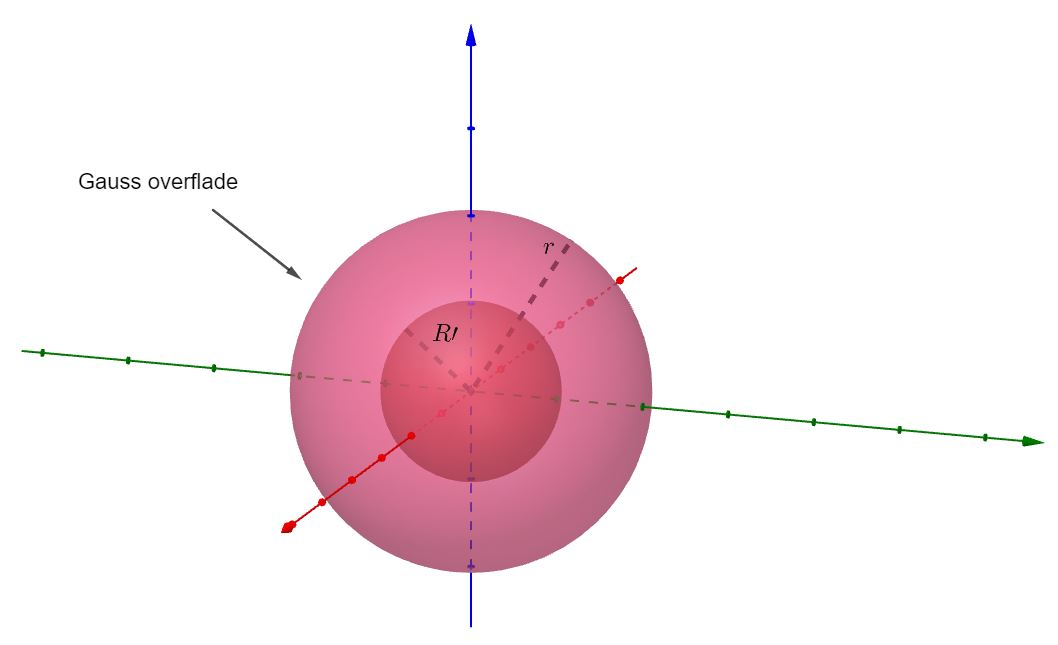
\includegraphics[scale=0.45]{Elektro/emfig/sym9.JPG}
    \caption{Gaussoverfladen har radius r, og er teknisk set en variable, der opfylder $r>R'$.}
    \label{em:fig:my_label}
\end{figure}
%
Nu mangler vi så at bestemme E-feltets størrelse. Vi starter igen med Gauss' lov, \cref{em:eq:gauss}:
%
\begin{align} \label{em:eq:gauss3}
    \oint \va{E}\cdot \dd{\va{a}}=\frac{Q_\textup{inde}}{\epsilon_0}.
\end{align}
%
Som Gaussoverflade, ville det være fornuftigt at bruge en sfærisk overflade (fordi, så er $\vu{r}\cdot \dd{\va{a}}=\dd{a}$) med radius $r>|R'|$. Indsætter vi \cref{em:eq:efeltstyrke_kugle} i \cref{em:eq:gauss3}, og anvender, at denne opstilling er rotationssymmetrisk, så skal $|E|$ være uændret langs vores Gauss-sfære (vi kan føre en testladning $q$ rundt på vores Gaussoverflade, og intet vil teknisk set ændre sig). Rotationssymmetrien skyldes, at sfærer kan drejes, så meget man har lyst til, uden at det ændrer noget. $|E|$ er dermed en konstant i integralet, som kan tages udenfor:
%
\begin{align}
    \oint \va{E}\cdot \dd{\va{a}} = |E|\oint\vu{r}\cdot\dd{\va{a}}.
\end{align}
%
Vi har også, at $\dd{\va{a}}$ peger i samme retning som $\vu{r}$ (altså, er $\vu{
r}\cdot\vu{n}=1$, hvor $\dd{\va{a}}=\vu{n}\dd{a}$). Tilbage får vi størrelsen af E-feltet gange arealet af en sfære, hvilket er
%
\begin{align}
    |E|\oint\dd{a}=|E|4\pi r^2=\frac{ Q_\textup{inde}}{\epsilon_0}.
\end{align}
%
Isolerer vi $|E|$, ser vi at
%
\begin{align}
    |E|=\frac{1}{4\pi \epsilon_0}\frac{Q_\textup{inde}}{r^2},
\end{align}
%
hvilket medfører at
%
\begin{align}
    \va{E}=|E|\va{r}=\frac{1}{4\pi \epsilon_0}\frac{Q_\textup{inde}}{r^2}\vu{r}.
\end{align}
%
Dette genkender vi fra er E-feltet for en punktpartikel med ladningen $Q_\textup{inde}$ (som vi plejer at kalde $q$), \cref{em:eq:e_felt_punktladninger}. Men dette er kun udenfor sfæren.

Hvad hvis vi gerne vil finde E-feltet inde i sfæren? Så skal vi sætte en Gaussoverflade inde i sfæren. Igen anvender vi også en sfære som Gaussoverflade. Vi kan da bruge samme argument som ovenover, og overbevise os selv om, at E-feltet nødvendigvis må pege radielt ud af, og være uændret under en rotation (sæt en testladning $q$ inde i sfæren og lav cirkler symmetrisk omkring den). Så vi har igen, at
%
\begin{align}
    |E|\oint\dd{a}=|E|4\pi r^2=\frac{ Q_\textup{inde}}{\epsilon_0}    
\end{align}
%
Denne gang indeslutter vores Gauss sfære ingenting -- tom luft! Derfor må $Q_\textup{inde}=0$, hvorfor $|E|=0$. Ligegyldigt hvor du placerer en testladning $Q$ inde i sfæren, så vil den ikke bevæge sig -- E-feltet og dermed kraften er 0! Dette har vi opdaget udelukkende ud fra symmetri.%, men igen er det overhovedet ikke et intuitivt svar (Man kan også vise dette vha. en længere integral udregning.)

Nu har vi set nogle eksempler på, hvordan vi igennem Gauss' lov, er kommet frem til E-feltet af en opstilling.
%
Kan man bare bruge Gauss' lov på alting? Nej, ikke rigtigt desværre. Gauss' lov er smart når E-feltet er symmetrisk: altså når E-feltet er ens flere forskellige steder. I eksemplerne har vi brugt, at vi ud fra symmetri kunne finde ud af hvilken retningen det elektriske felt har overalt i rummet. Kan man ikke det, så bliver det svært, at bruge Gauss' lov til at bestemme det elektriske felt.

Har man dog et symmetrisk E-felt, så er den generelle fremgangsmåde til at udregne E-feltet det følgende:
%
\begin{itemize}
    \item Identificer \emph{retningen} af E-feltet: dette kan gøres med udgangspunkt i Coulombs lov og symmetri.
    \item Placer en \emph{Gaussoverflade} i dit E-felt, hvor overfladens arealvektor $\dd{\va{a}}$ enten er parallel eller vinkelret med E-feltet.
    \item Udregn arealet af de sider på din Gaussoverflade, som er parallel med E-feltet. Resten giver nul.
\end{itemize}

Heldigvis findes der kun tre forskellige, almindelige symmetrier (plan-, sfærisk samt cylinderisk symmetrisk) så når først vi kender dem, er det ikke så slemt. Vi har gennemgået to af symmetrierne, og så får I lov til at udregne den sidste selv!

\newpage
\section{Magnetostatik}
Tillykke, du er kommet sikkert igennem en introduktion til elektrostatik, og du er nu påklædt til at komme videre til næste trin: magnetostatik! Vi har set en masse på E-felter forårsaget af vekselvirkninger imellem ladninger: indtil videre har alle disse ladninger stået stille. Når ladninger bevæger sig, bliver der dannet et andet slags felt: dem kalder vi magnetiske felter, eller B-felter\footnote{Hvorfor er magnetiske felter ikke M-felter, når elektriske felter er E-felter? Da James Clerk Maxwell fremsagde sin teori indenfor elektromagnetismen, startede han vidst bare fra en ende af i alfabetet, også var det magnetiske felt altså bare nr. 2 i rækken. A er typisk reserveret til noget andet i elektromagnetisme, som vi dog ikke vil komme ind på.}. \\ 

Nu skal vi i gang med at undersøge hvad der sker, hvis en ladning er i bevægelse. Her vil vi specifikt se på ladninger i en konstant eller \emph{jævn} bevægelse, og altså ikke bare punktladninger, der bevæger sig. Hvis ladningerne accelerere vil det medføre dynamiske felter, hvor B og E-felterne vekselvirker med hinanden. En jævn bevægelse svarer til, at der ikke er noget ladning som ``hober sig op'' eller ``fortyndes'' forskellige steder, der er en konstant mængde ladning for ethvert stykke og en konstant hastighed, som vi kalder strømtyrken. Det svarer til at den magnetiske flux (flux fra det magnetiske felt, ikke det elektriske!) er konstant.
Magnetostatikken bygger på mange af de samme principper som elektrostatikken, og derfor vil vi ikke gå lige så meget i dybden i dette emne: det vigtigste er bare at I ser lighederne, og vi benytter os af denne symmetri.

\subsection{Strømtæthed}
Strøm er faktisk ladning i en jævn bevægelse. Så mens E-felter afhænger af ladningstætheder, som vi så i afsnittet tidligere, så afhænger B-felter af strømtætheden. Det vil sige hvor høj en tæthed eller densitet af ladning, som bevæger sig med en givet hastighed. Ladningerne udstrækkes også i forskellige dimensioner, og derved får vi også forskellige typer strømdensiteter:
%
\begin{itemize}
    \item \emph{Strøm i en linje, $\va{I}$}: En linjeladning på $\lambda$ bevæger sig med hastigheden $\va{v}$. ($\va{I}=\lambda\va{v}$)
    \item \emph{Strøm på et areal, $\va{K}$}: her er ladningen ligeligt fordelt på en flade med en overfladeladningstæthed $\sigma$, som bevæger sig med hastigheden $\va{v}$. ($\va{K}=\sigma\va{v}$)
    \item \emph{Ladning i et volumen, $\va{J}$}: ladningen er fordel ligeligt på en rumlig figur med en volumeladningstæthed $\rho$, som ligeledes bevæger sig med hastigheden $\va{v}$. ($\va{J}=\rho\va{v}$)
\end{itemize}
%
Bemærk at vi ikke kan have en enkelt punktladning, da det ikke er muligt at have en jævn strømning bestående af et enkelt element. Så ville densiteten netop være ekstremt skævt fordelt i rummet, så en ladning i jævn bevægelse, vil ikke danne et statisk felt, som er det eneste typer vi undersøger her på campen\footnote{Magneto- og elektrostatik er egentlig en forsimpling af elektrodynamik. I virkeligheden er det svært at have en ladning som står helt stille, eller en ladningsfordeling, som bevæger sig helt jævnt: men de to teorier fremhæver det helt fundamentale bag elektrodynamikken, og ofte er det gode nok approksimationer.}. Strøm svarer til ladning per tid, altså et mål for hvor hurtigt ladningerne bevæger sig. For de tre eksempler har vi:
%
\begin{align*}
    I&=\lambda \va{v}\\
    I&=\int \sigma \va{v} \dd{l}_\perp\\
    I& = \int \rho \va{v} \dd{a}_\perp
\end{align*}
%
Den jævne bevægelse kan rent matematisk opskrives som en ladning, der ikke ændrer sig over tid:
%
\begin{align}
    \pdv{\va J}{t} = \pdv{\va I}{t} = 0.
\end{align}
%
\begin{figure}[]
    \centering
    \includegraphics[scale=0.675]{Elektro/emfig/Tætheder.png}
    \caption{En illustration af de forskellige måder ladninger kan bevæge sig i en jævn strøm.}
    \label{em:fig:tetheder}
\end{figure}

\subsection{Biot-Savarts lov}
Ligesom elektrostatikken har Coulombs lov til at beskrive kraften mellem elektriske ladninger, så har magnetostatikken Biot-Savarts lov, til at udregne B-feltet i et givet punkt med afstanden $\va{R}$ fra en samling af ladninger med strømstyrken $\va{I}$:
%
\begin{align}\label{em:eq:biot-savart}
    \va{B}=\frac{\mu_0}{4\pi}\int \frac{\va{I}\cross \va{R}}{R^2} \dd{l'}.
\end{align}
%
$\va{R}$ vil altid være den korteste afstand mellem det lille stykke af ledningen til punktet, vi ønsker at kende B-feltet i, mens $\mu_0$ er en konstant. Biot-Savarts lov danner et fundament for magnetiske felter.

I hvilken retning peger B-feltet så? Her skal vi frem med højre hånd, da det er krydsproduktet inde i tælleren i \cref{em:eq:biot-savart}, som afgører retningen af B-feltet.
%
Det betyder at B-feltet vil pege vinkelret på strømmens retning og den vektor, der strækker sig den korteste afstand fra samlingen af ladninger til $\va{R}$, som er punktet hvori vi gerne vil kende B-feltet. Derudover vil $1/R^2$-ledet medføre at jo længere væk du kommer fra strømmen, desto lavere er styrken af B-feltet. B-feltet afhænger af, hvor vi evaluere det (med $\va{R}$-vektoren efter samme princip som i elektrostatik med Coulombs lov), så vi er nød til at se på et eksempel for at få en bedre intuition for det samlede B-felt og ikke blot i et enkelt punkt.
%
\begin{figure}[]
    \centering
    \begin{tikzpicture}[line width=2.5pt]
		\node[anchor=south west,inner sep=0] at (0,0)
		{ 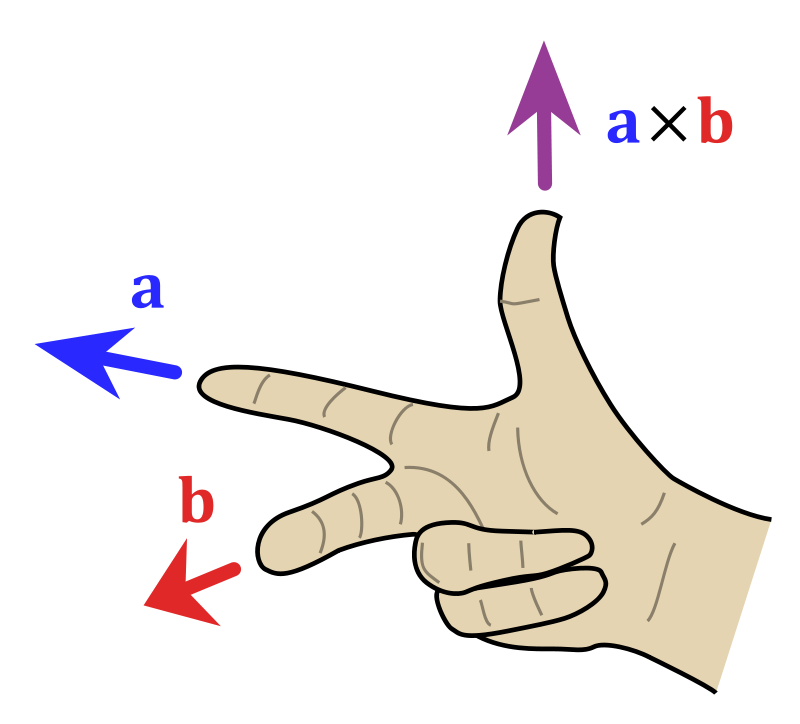
\includegraphics[width=0.5 \textwidth]{Matematik/matfig/righthandmat.png} };
		% Nu indsættes hvide rektangler over originalteksten, som erstattes af vores egen
		\coordinate (a) at (1.25,4.1);
		\fill[white] (a) rectangle ++(1,1);
        \draw[blue] (a) node[anchor=south west]{\HUGE $\va{R}$};
		%
		\coordinate (b) at (1.7,2);
		\fill[white] (b) rectangle ++(0.9,0.9);
        \draw[red] (b) node[anchor=south west]{\HUGE $\va{B}$};
		%		
		\coordinate (c) at (6,5.8);
		\fill[white] (c) rectangle ++(5,2);
        \draw[color=blue!50!red] (c) node[anchor=south west]{\HUGE $\va{I}$};
	\end{tikzpicture}
    % 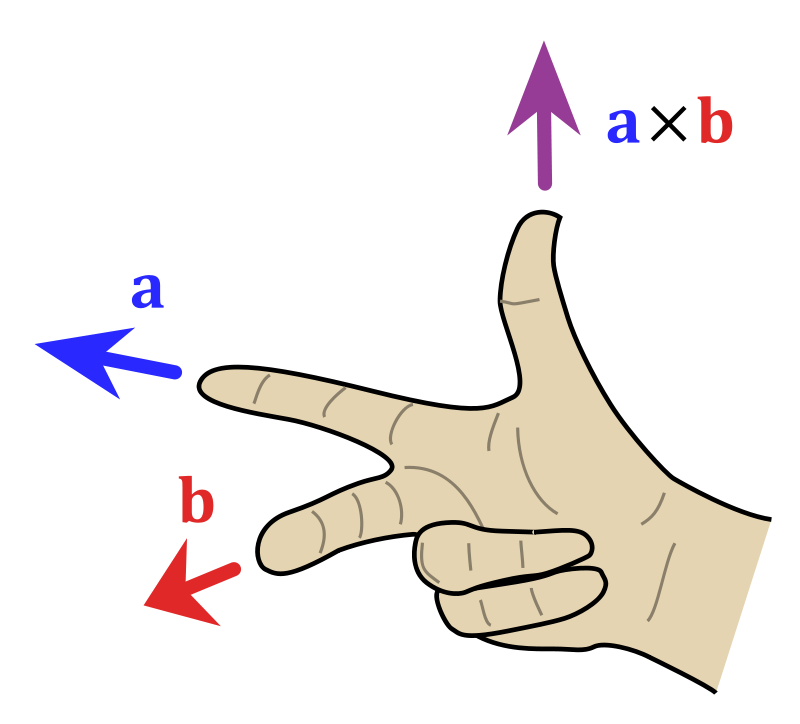
\includegraphics[width = 0.7 \textwidth]{Matematik/matfig/righthandmat.png}
    \caption{Højrehåndsreglen fortæller hvilken retning B-feltet vil være ud fra strømmens retning og vektoren $\va{R}$. Kilde: \cite{RighthandRuleWikipedia}.}
    \label{em:fig:right_hand_rule_mat}
\end{figure}
%

\subsection{Symmetrier}
Heldigvis kan vi endnu engang benytte os af symmetrien til at opnå et større billede af, hvordan B-feltet ser ud. Ligesom Gauss' lov er en vej til E-feltet, i stedet for Coulombs lov, så har vi \emph{Amperes lov}, der kan bruges i stedet for Biot-Savarts lov. I dette afsnit vil vi udlede denne lov, og her skal vi altså bruge en fysikers yndlingstilgang: symmetrier!

\subsubsection{Amperes lov}
For at frembringe en mere simpel metode, så vælger vi ligesom i elektrostatik-afsnittet at tage udgangspunkt det simpleste eksempel: en jævn strøm af ladninger i en ret linje gående fra venstre til højre: en ledning. Så vi vil undersøge styrken og retningen af det magnetiske felt fra afstanden $R$, som svarer til vores vektor $\va{R}$.

For at finde det magnetiske felt, om en linje, skal vi udregne krydsproduktet fra strømmens retning\footnote{Det ser måske støjst ud af angive strømstyrken som en vektor, men det er netop fordi vi også er interesseret i dens retning.} $\va{I}$ og vektoren $\va{R}$ fra ledningen til testladningens placering. Da de to vektorer netop er vinkelrette på hinanden, vil de også være vinkelrette med B-feltet.
Strømstyrken har samme styrke og retning hele vejen, men afstanden vil være anderledes, så derfor vil styrken af magnetfeltet variere, men retningen vil altid være den samme: nemlig vinkelret på ledningen og $\va{R}$. Systemet er således symmetrisk, fordi vinklen mellem $\va{I}$ og $\va{R}$ altid vil være den samme. Retningen på krydsproduktet kan findes med højrehåndsreglen i \cref{em:fig:right_hand_rule_mat} eller den i \cref{em:fig:right_hand_rule_mat2} -- de er ækvivalente.

\begin{figure}[]
    \begin{minipage}{0.5\textwidth}
    \centering
    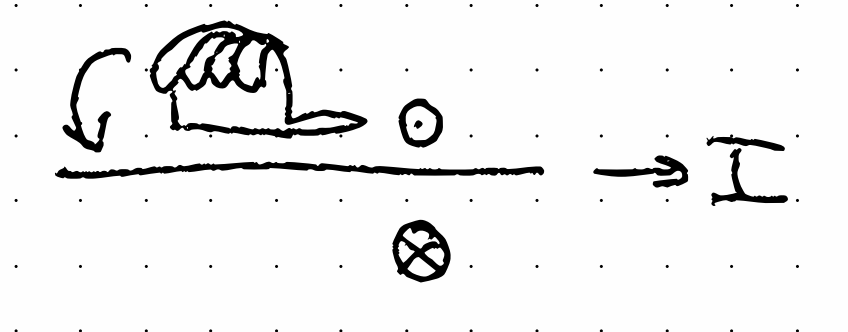
\includegraphics[scale=0.7]{Elektro/emfig/hojrehand.png}
    \label{em:fig:hojre1}
    \end{minipage}
    \begin{minipage}{0.5\textwidth}
    \centering
    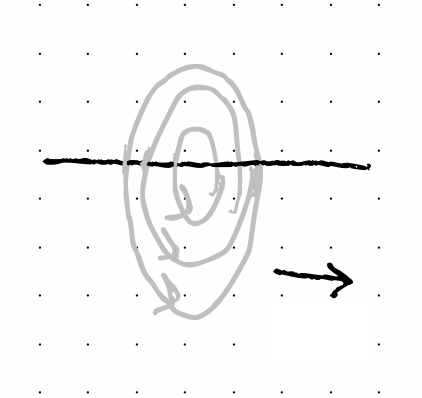
\includegraphics[scale=0.8]{Elektro/emfig/b-linje.png}
    \label{em:fig:hojre2}
    \end{minipage}\hfill
    \caption{Ud fra højrehåndsreglen kan du finde retningen af B-feltet. Placer din tommelfinger langs strømmen hvortil B-feltet bevæger sig rundt om i cirkler i retningen af resten af dine fingre som vist til højre. Den højrehåndsregel, der er vist her, er ækvivalent til den i \cref{em:fig:right_hand_rule_mat}, men den er god til netop magnetfeltet omkring en lednings retning.}
    \label{em:fig:right_hand_rule_mat2}
\end{figure}

Nu har vi styr på retningen af magnetfeltet, men hvad med størrelsen? Her er vi nød til at summe alle linjestykkerne sammen i integralet i Biot-Savarts lov, og det kan hurtigt blive meget snørklet. Det er her vi skal benytte os af Amperes lov, som ser ud som følgende: 
%
\begin{align} \label{em:eq:ampere}
    \oint \va B \cdot \dd{\va{l}} = \mu_0 I_\mathrm{inde}.
\end{align}
%
Den betyder, at hvis vi tegner en løkke rundt om en jævn strøm (f.eks. fra en ledning), så vil størrelsen af B-feltet svare til størrelsen af den indelukkede strøm ganget med $\mu_0$ -- konstanten vi nævnte tidligere. Løkken kaldes i dette tilfælde for en \emph{Ampereløkke}. Denne tanke er illustreret i \cref{em:fig:ampere}.

\begin{figure}[]
    \centering
    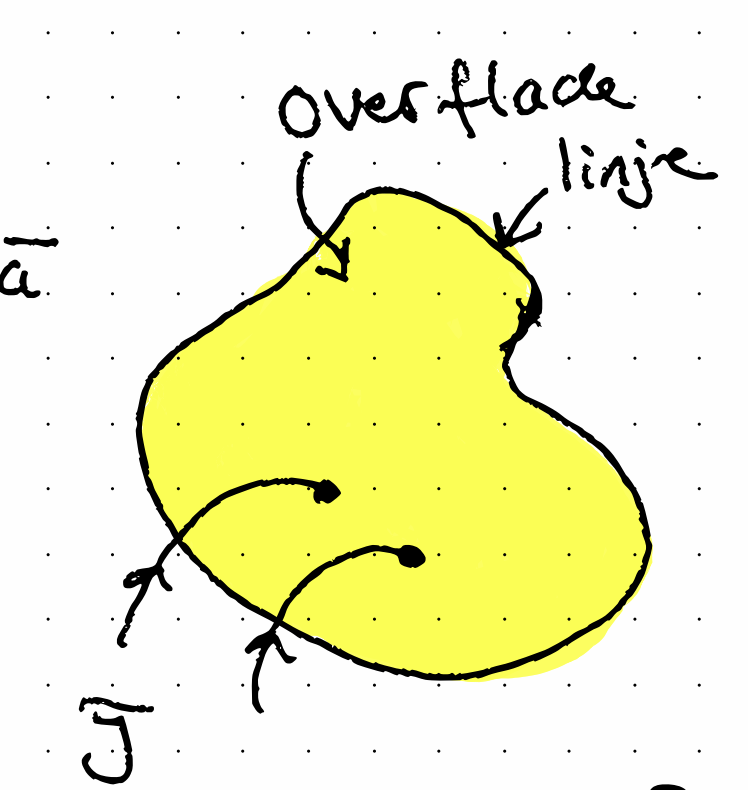
\includegraphics[scale=0.42]{Elektro/emfig/ampere.png}
    \caption{To ledninger med strømmen $\va{J}$, som skærer ind i en Ampereløkke, hvis overflade er markeret med gul.}
    \label{em:fig:ampere}
\end{figure}

Vi vil ikke gå lige så meget i dybden denne gang med intuitionen bag Amperes lov, men vi vil komme med de vigtige konklusioner. Tegner du din løkke om din strøm $\va{I}$, så løkken er vinkelret med B-feltet, så kan vi omskrive integralet til at kunne udregne omkredse/overfladeareal (hvor det var areal/volumen ved Gauss' lov):
%
\begin{align}
    \oint \va{B} \cdot \dd{\va{l}} = |B|\oint \dd{\va{l}}.
\end{align}
%
Det giver også den samlede fremgangsmåde til at finde B-feltet: 
%
\begin{itemize}
    \item Identificer \emph{retningen} af B-feltet: dette gøres ud fra højrehåndsreglen for krydsproduktet $\va{I}\cross \va{R}$. Se \cref{em:fig:right_hand_rule_mat,em:fig:right_hand_rule_mat2}.
    \item Placer en \emph{Ampereløkke} i dit B-felt, hvor hver af løkkens linjestykke $\dd{l}'$ enten er parallel eller vinkelret med B-feltet.
    \item Udregn længden af de sider på din Ampereløkke som er parallel med B-feltet og ignorer resten.
\end{itemize}


\begin{figure}[]
    \centering
    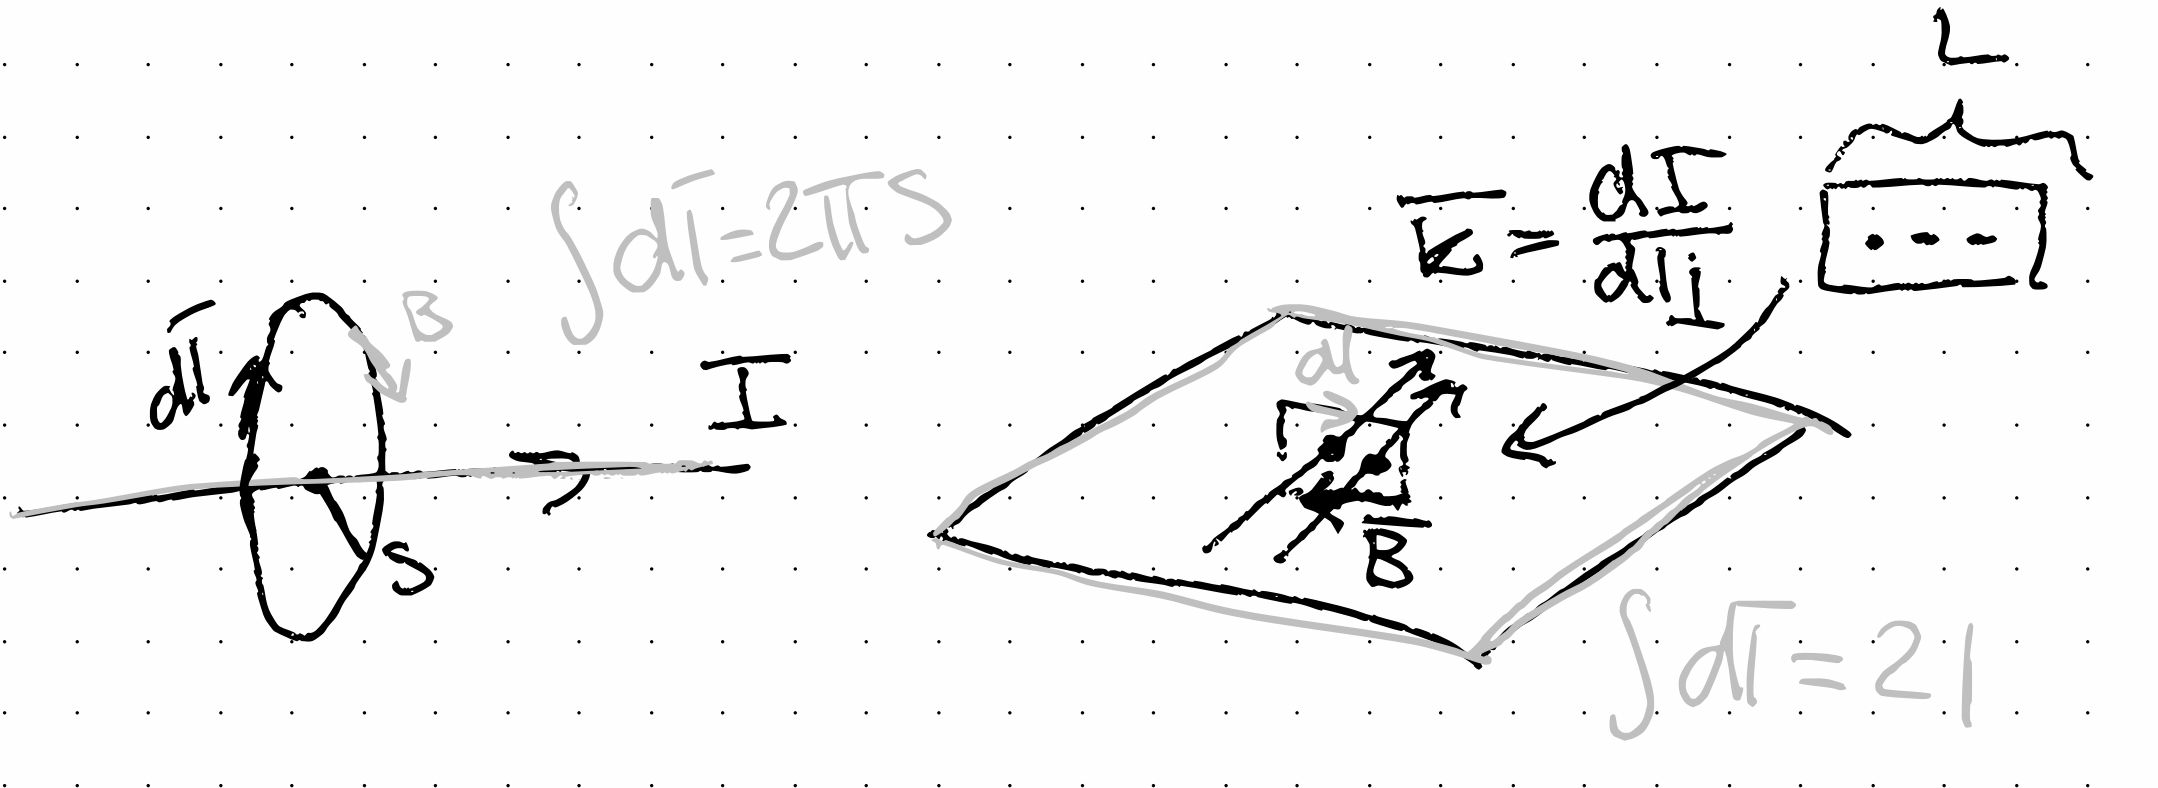
\includegraphics[scale=0.4]{Elektro/emfig/sym-B.png}
    \caption{To eksempler på brugen af Amperes lov. Til venstre: en uendelig lang ledning. Til højre: en uendelig lang flade (dette eksempel er mest med for sjov).}
    \label{em:fig:bsym}
\end{figure}
%
\subsubsection{Eksempler på symmetrier}
Lad os nu rent faktisk udregne B-feltet af en uendelig lang ledning med strømmen $\va{I}$. Først skal vi bedømme retningen af B-feltet: vi ved heldigvis allerede at B-feltet bevæger sig i cirkler rundt om ledningen. Næste skridt er at tegne en Ampereløkke. For at Ampereløkkens linjestykker $\dd{\va{l}}$ altid er parallel med B-feltet, må den ligeledes være en cirkel rundt om ledningen, som vist i \cref{em:fig:bsym}. 

Efter vi har valgt Ampereløkken skal vi nu udregne den samlede længde af løkken, da den altid er parallel med B-feltet. Dette indsættes i Amperes lov, \cref{em:eq:ampere}
%
\begin{align} \label{em:eq:ampere2}
    \oint \va B \cdot \dd{\va{l}} = |B|\oint \dd{\va{l}} = |B| 2 \pi R =  \mu_0 I_\mathrm{inde},
\end{align}
%
hvori vi kan isolere størrelsen af B-feltet:
%
\begin{align}
    |B| = \frac{\mu_0 I}{2 \pi R}.
\end{align}
%
Her kan vi også se, at B-feltet aftager i styrke, når vi bevæger os længere væk fra ledningen. Retningen er stadig rundt omkring ledningen. Så vi har formået at udregne B-feltet af en ledning helt uden af bruge Biot-Savarts lov -- det er da ret sejt! I opgaverne vil I have mulighed for selv at prøve at gennemskue retningen af B-felter som følge af forskellige konfigurationer af strømtætheder, og derefter udregne størrelsen.

\newpage
\section{Potentialer og konservative felter (Bonus afsnit)}
Vi har indtil videre opdaget, at ved at udregne E-felter kan vi ligeledes finde en kraftpåvirkning som en givet ladning ville påvirke en testladning $q$ med. Vi har endda fundet et vildt essentielt værktøj, nemlig Gauss' lov, som er helt afgørende for at udregne E-felter. Lad os nu dykke endnu dybere ned i elektrostatikkens gåder og se hvordan det vil være at bevæge sig rundt i E-feltet - altså hvordan vi kan bevæge os fra punkt $\va{a}$ til $\va{b}$ i det elektriske felt $\va{E}$. For at rykke en testladning $Q$ i et elektrisk felt $\va{E}$ udspændt af fra en ladning $q$, kræver det energi og derved er det et arbejde $W$:
%
\begin{align}
    W_{ab}=-Q\int^{\va{a}}_{\va{b}} \va{E}\cdot d\va{l}
\end{align}
%
Da det elektriske felt kun afhænger af r-koordinatet, så kan vi omskrive integralet og derefter løse det.
%
\begin{align}
    W_{ab}=-Q\int^{\va{a}}_{\va{b}} \va{E}\cdot d\va{l} = -\frac{Q}{4\pi \epsilon_0} \int \frac{-1}{r^2} dr = \frac{Q}{4\pi \epsilon_0} \left[\frac{q}{r} \right]^{r_b}_{r_a} = -\frac{Q}{4\pi \epsilon_0} \left(\frac{q}{r_a}-\frac{q}{r_b} \right) \label{konservativ}
\end{align}
%
Okay, så det er et meget interessant svar. Det betyder nemlig, at hvis vi nu bevæger testladningen rundt i hele det elektrostatiske felt også derefter slutter af ved det samme sted, altså bevæger os rundt i en lukket kurve, så vil linjeintegralet give 0! Dette faktum viser vi med et lukket integrale: 
%
\begin{align}
    \oint \va{E} \cdot d\va{l} = 0
\end{align}
%
Lad os sige at det var en testladning $q$ som bevægelse sig, så vil arbejdet svare til kraft gange strækning $W=F\cdot\delta s$. Da vi ved at kraften svarer til dette elektriske felt gange testladningen $\va{F}=G\va{E}$ mens strækningen er dette linjeintegrale så får vi: 
%
\begin{align}
    W=-Q\oint \va{E} \cdot d\va{l} = 0
\end{align}
%
Hvoraf det negative fortegn stammer fra at vi udregner det arbejde \emph{du} skal udføre for at bevæge testladningen.

Det betyder altså, at ligegyldigt hvordan du ville bevæge dig rundt i feltet, så vil det totale arbejde være nul! Hvordan kan det lige være at det ikke kræver energi at rykke vores testladning rundt? Det er faktisk et meget normalt fænomen, det skyldes nemlig at vi den elektriske kraft er konservativ. Tyngdekraften er også konservativ, og der gælder præcis det samme! \footnote{Hvis du holder en kasse i hånden og rykker den op og ned, men kassen ender det samme sted, så har du ikke udført et arbejde på kassen.} \\

Hvis vi nu går tilbage til vores to punkter $\va{a}$ og $\va{b}$, så vil det også sige, at ligegyldigt hvordan vi går fra det ene punkt til det andet, så vil det kræve den samme mængde energi: \cref{konservativ} afhænger kun af slutpunkterne og ikke dem indimellem. Dette svarer også til, at der ikke er nogen veje som er bedre end andre: eller nogen som koster mere energi. Faktisk så betyder det, at det ikke kræver noget som helst energi, hvis bare ladningen ender det samme sted som den starterede. Dette kan også tolkes som, at kraften ikke har nogen friktion. Dette kan opsummeres: 

\begin{itemize}
    \item Elektrostatiske felter har ingen intern rotation eller friktion. Hvis du placere en lille pind i ethvert punkt sted i det elektriske felt, vil det altså ikke rotere eller bruge energi (konservativt felt). 
    \item Elektrostatiske felter kan strømme mindre eller mere flux igennem en lukket område, hvis der er en eller anden form for ladning som indeni (Gauss' lov)
\end{itemize}

En vigtig konsekvens af dette er, at ethvert elektrostatisk felt kan beskrives ud fra en ganske almindelig funktion, kaldet potentialet:
%
\begin{align}
    \va{E}=-\nabla V
\end{align}
%
Vi vil ikke udlede hvorfor dette er tilfældet, men det er en direkte udledning af at elektrostatiske felter er konservative. Potentialer er enormt vigtige i fysik og ofte er det nemmere at udregne E-felter ud fra potentialet. I vil helt sikkert støde på potentialer og meget mere til, hvis I starter på fysikstudiet!



\nocite{griffithsIntroductionElectrodynamics2018}
\nocite{youngSearsZemanskyUniversity2016}

\end{document}